%versi 2 (8-10-2016)
\chapter{Landasan Teori}

Pada bab ini dijelaskan beberapa dasar teori dan \textit{framework} yang digunakan dalam merancang dan membangun perangkat lunak untuk melakukan klasifikasi Naive Bayes pada sistem terdistribusi Hadoop. Dasar teori yang dijelaskan pada bab ini meliputi: (1) Penambangan data ; (2) \textit{Big data} ; (3) Sistem terdistribusi Hadoop ; (4) \textit{Naive Bayes classification} ; (5) \textit{Spring framework, Maven, } dan \textit{Thymeleaf}. \\

\section{Penambangan Data}

\subsection{Definisi Penambangan Data}
Penambangan data (\textit{data mining}) adalah suatu proses untuk menemukan suatu
pengetahuan atau informasi yang berguna dari data berskala besar. Sering juga
disebut sebagai bagian proses KDD (\textit{Knowledge Discovery in Databases}) \cite{Piateski:1991:KDD:583310}. \textit{Data mining} melakukan pemecahan masalah dengan menganalisis data yang ada di dalam basis data dan sering juga didefinisikan sebagai proses menemukan pola dalam data. Proses tersebut harus otomatis atau semi-otomatis dan pola yang ditemukan harus bermakna \cite{DataMiningIntro:2015}.

\textit{Data mining} secara umum adalah mengenai pembuatan sebuah model. Suatu model dari teknik \textit{data mining} merupakan suatu algoritma atau sekumpulan aturan yang menghubungkan suatu input data set dengan hasil dari output yang diinginkan. Sebuah model yang dibuat menggunakan teknik \textit{data mining} dapat memiliki tingkat akurasi yang tinggi atau rendah. Hal tersebut bergantung pada pemilihan data yang digunakan sebagai input dan output yang harus memiliki hubungan \cite{book:339389}.

\subsection{Tugas Yang Dapat Dilakukan Oleh \textit{Data Mining}}

Beberapa tugas - tugas yang dapat diselesaikan menggunakan \textit{data mining} diantaranya adalah:

\begin{itemize}
	\item \textit{Classification}
	\item \textit{Estimation}
	\item \textit{Affinity grouping}
	\item \textit{Clustering}
	\item \textit{Description and profiling}
\end{itemize}

Pada bagian ini, hanya dijelaskan mengenai teknik klasifikasi dan klustering. Karena, kedua algoritma ini memiliki sistem pembelajaran yang berbeda. Sehingga, dapat memudahkan dalam melihat perbedaan yang dimiliki oleh teknik tersebut.

\begin{enumerate}
	\item{\textit{Classification}\cite{book:339389}}\\
	Klasifikasi juga merupakan algoritma mesin learning yang bersifat terawasi (\textit{supervised learning}). Dimana dalam pembuatan modelnya diperlukan data latih (umumnya disebut sebagai \textit{data training}) terlebih dahulu untuk dijadikan acuan dalam melakukan klasifikasi data.
	
	Algoritma klasifikasi adalah salah satu tugas data mining yang paling umum, tampaknya dewasa ini hal tersebut menjadi penting bagi perusahaan - perusahaan yang memiliki data transaksi. Di samping perusahaan, kita juga sebagai manusia secara terus-menerus mengklasifikasikan, mengkategorikan, dan melakukan penilaian terhadap sesuatu. 
	
	Klasifikasi memeriksa atribut dari objek baru yang diberikan dan dilemparkan ke dalam model standar klasifikasi yang sudah ada. Objek yang diklasifikasikan umumnya diwakili oleh \textit{record - record} dalam tabel database atau file, dan tindakan klasifikasi terdiri dari menambahkan kolom (\textit{field}) baru dengan kode kelas (\textit{kelompok}) dari beberapa jenis kelas. Tugas kita adalah untuk membangun model dari beberapa jenis \textit{dataset} yang dapat diterapkan pada data yang belum terklasifikasi untuk diklasifikasikan ke dalam kelompok yang sudah ada. Berikut merupakan beberapa contoh dari penerapan teknik klasifikasi:
\begin{itemize}
	\item Klasifikasi calon pengguna kartu kredit yang memiliki resiko rendah, sedang, atau tinggi.
	\item Memilih konten yang ditampilkan pada halaman Web.
	\item Menentukan nomor telepon sesuai dengan mesin faks.
	\item Menentukan potensi dari klaim asuransi palsu.
\end{itemize}
	\item{\textit{Clustering}\cite{book:339389}} \\
	Klustering juga merupakan algoritma mesin learning yang bersifat tidak terawasi (\textit{unsupervised learning}). Berbeda dengan teknik klasifikasi, dalam pembuatan model teknik ini tidak diperlukan data latih (umumnya disebut sebagai \textit{data training}) terlebih dahulu. Klustering hanya melakukan pengelompokkan sejumlah data yang memiliki kemiripan yang tinggi. Berikut merupakan beberapa contoh dari penerapan teknik klustering:
\begin{itemize}
	\item Mencari distribusi penjualan suatu barang tertentu berdasarkan lokasi tempat tinggal konsumen dan tingkat penghasilan konsumen.
	%\item Mencari distribusi penjualan suatu barang tertentu berdasarkan tingkat penghasilan konsumen.
	\item Mengetahui rentang umur yang paling banyak melakukan transaksi terhadap suatu barang (melakukan pembelian barang tersebut) untuk dijadikan \textit{targeted marketing}.
\end{itemize}
\end{enumerate}

\subsection{Langkah - langkah Penambangan Data}

\begin{figure}[h]
	\centering
	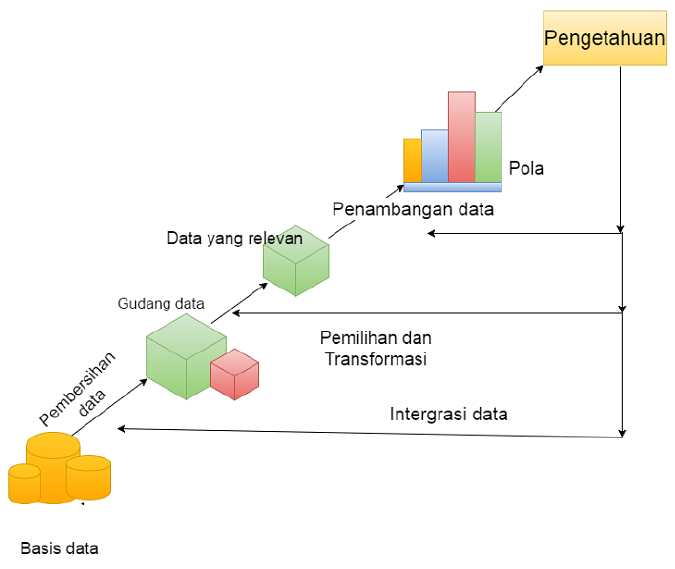
\includegraphics[scale=0.7]{GambarIO/langkah-data-mining}
	\caption[Langkah Penambangan Data]{Langkah Penambangan Data}
	\label{fig:Langkah Penambangan Data}
\end{figure}

Gambar~\ref{fig:Langkah Penambangan Data} menyatakan langkah-langkah untuk menemukan pengetahuan dan proses-proses pengolahan data. Gambar~\ref{fig:Langkah Penambangan Data} juga menyatakan bahwa setelah meraih pengetahuan, proses pencarian pengetahuan lebih lanjut juga dapat dilakukan kembali. Lihat anak panah pada Gambar~\ref{fig:Langkah Penambangan Data} yang merujuk pada langkah-langkah yang dapat dilakukan kembali untuk mendapatkan pengetahuan yang lebih mendalam. Berikut adalah proses-proses yang harus dilakukan dalam mencari pengetahuan baru \cite{DataMiningIntro:2015}:

\begin{itemize}
	\item{Pembersihan Data} \\
	Pembersihan data adalah fase yang membuang data yang tidak berguna (noise) dan data yang tidak relevan.
	\item{Integrasi data} \\
	Pada fase ini, beberapa sumber data yang heterogen digabungkan menjadi satu.
	\item{Pemilihan Data} \\
	Fase ini adalah fase di mana data dipilih, data yang relevan dipilih dari koleksi data pada fase sebelumnya.
	\item{Transformasi Data} \\
	Pada fase ini data yang dipilih ditransformasi sehingga memiliki bentuk yang layak untuk ditambang.
	\item{Penambangan Data} \\
	Fase ini adalah fase di mana teknik-teknik penambangan digunakan untuk mencari pola yang memiliki potensi.
	\item{Evaluasi Pola} \\
	Pada fase ini, pola yang menarik diidentifikasi dan dianalisis sehingga dapat menghasilkan pengetahuan yang baru.
	\item{Penyimpulan Pengetahuan} \\
	Fase terakhir ini adalah fase di mana pengetahuan yang baru ditemukan itu direpresentasikan kepada pengguna.
\end{itemize}

\section{{\it Big Data}}

\subsection{Definisi {\it Big Data}}
{\it Big Data} merupakan suatu terminologi modern untuk sekumpulan data yang memiliki kesulitan tersendiri untuk diproses dengan cara tradisional (menggunakan satu buah komputer) \cite{zikopoulos2011understanding}. Dewasa ini perusahaan - perusahaan tengah menghadapi tantangan - tantangan yang ada pada {\it Big Data}, karena pertumbuhan data yang sudah semakin cepat dan jumlah pengguna internet yang semakin menaik setiap saat. Mereka mendapatkan akses pada data/informasi tersebut tetapi tidak tahu cara mengambil informasi yang berguna pada data tersebut karena format dari data tersebut yang semi bahkan ada yang tidak terstruktur dan juga ukuran-nya yang sangat besar ; Cukup kebingungan apakah data tersebut berguna apabila terus disimpan. Karena, dapat dapat menyebabkan {\it memory overload}.

{\it Big Data} tidak melulu berasal dari internet, di dalam kehidupan kita sehari - hari sering kali kita berurusan dengan data, seperti data pada sensor sidik jari ketika absensi, data pembelian pada supermarket, data sensor kelembaban udara pada 10 tahun terakhir untuk memprediksi cuaca, kenaikan dan penurunan harga saham, {\it bitcoin}, dsb. {\it Big Data} menjadi topik yang diminati karena dengan data yang begitu banyak, dapat diteliti pola yang terjadi pada data tersebut selama beberapa kurun waktu tertentu untuk digunakan dalam menganalisis data dan membuat keputusan serta memberikan prediksi kemunculan data berikutnya dengan tingkat akurasi yang tinggi berdasarkan data yang dipelajari. Perusahaan - perusahaan saat ini tengah memulai untuk mengumpulkan setiap data yang dapat mereka peroleh dari {\it customer} untuk melihat pola perilaku dari {\it customer} mereka dan membuat keputusan yang dapat menguntungkan perusahaan berdasarkan hal tersebut. Tentu saja hal ini tidak dapat dilakukan menggunakan teknik komputasi yang tradisional (menggunakan satu buah komputer berteknologi tinggi), karena biaya dan waktu yang terlalu mahal dan lama.

\subsection{Karakteristik {\it Big Data}}

 Tiga hal terpenting yang menjadi pokok permasalahan dalam {\it Big Data} adalah : 
\begin{enumerate}
	\item{Mengolah data yang berjumlah sangat besar} \\
	Ukuran data yang menjadi tantangan pada big data saat ini sangat besar, mulai dari \textit{GigaByte} bahkan bisa mencapai puluhan \textit{PetaByte}.
	\item{Mengolah data yang memiliki tipe sangat bermacam - macam / variatif} \\
	Tipe dari data pada \textit{big data} sangat bermacam - macam. seperti: (1) angka, (2) tanggal, (3) \textit{string}\footnote{\textit{String} dalam pemrograman komputer adalah sebuah deret simbol. Tipe data string adalah tipe data yang digunakan untuk menyimpan barisan karakter}
	\item{Mengolah data dengan performa yang optimal}\\
	Tantangan yang terakhir pada \textit{big data} adalah kebutuhan untuk mengolah \textit{big data} dengan waktu dan sumber daya yang se-optimal dan se-efisien mungkin.
\end{enumerate}

Berikut merupakan beberapa contoh \textit{big data} dan pemanfaatannya di berbagai bidang \cite{JNetwork2012introductionBigData}:
\begin{enumerate}
	\item Pada bidang penerbangan dan transportasi, big data didapat dari data konsumsi bahan bakar dan pola lalu lintas di setiap armada secara nyata untuk meningkatkan efisiensi dalam penggunaan bahan bakar.
	\item Pada sektor kesehatan, big data didapat dari berbagai catatan kesehatan elektronik pasien dari berbagai sumber, perawatan, demografi dan pencatatan khasiat obat sehingga dapat memberikan proses pengembangan obat yang lebih efisien dan cepat.
	\item Pada sektor telekomunikasi, big data didapat dari penggunaan dan permintaan pengguna sehingga perusahaan telekomunikasi dapat menganalisis perilaku pengguna dan pola permintaan tersebut.
	\item Pada sektor media dan hiburan, big data didapat dari penggunaan media dan hiburan sehingga dapat dimanfaatkan untuk membantu pengambilan keputusan dan analisis prediktif dari penggunaan media dan hiburan tersebut.
\end{enumerate}


\section{Sistem Terdistribusi Hadoop}
	\subsection{Definisi Hadoop}
	Apache Hadoop merupakan platform \textit{open source} yang didirikan pada tahun 2006 untuk melakukan analisis pada big data. Hadoop merupakan software framework open source yang dapat menangani pertumbuhan jumlah data yang tinggi tanpa mempengaruhi performa kinerja-nya dengan sistem komputasi yang terdistribusi pada beberapa mesin yang dimiliki oleh Hadoop secara efisien \cite{Lam:2010:HA:1965594}. Hadoop terinspirasi dari MapReduce milik Google\cite{GoogleMR:2004} dan Google File System (GFS) \cite{GFS:2003}. \\
	Hadoop cluster\footnote{cluster merupakan sekelompok server} terdiri dari 2 jenis \textit{node}\footnote{\textit{node} merupakan istilah teknik yang digunakan untuk menjelaskan suatu mesin atau komputer} yaitu \textit{Master Node} yang terdiri dari \textit{Namenode} dan \textit{Jobtracker daemon}\footnote{Daemon merupakan isitlah teknis yang digunakan untuk menjelaskan suatu proses yang berjalan secara background pada mesin linux} dan \textit{Slave Node} yang terdiri dari \textit{Datanode} dan \textit{Task Tracker}.
	
	\begin{figure}[ht]
			\centering
			\includegraphics[scale=0.7]{GambarIO/Master-Slave-Hadoop}
			\caption[Arsitektur master-slave]{Arsitektur master-slave}
			\label{fig:Arsitektur master-slave}
		\end{figure}
	
	\subsection{Fitur - fitur dari \textit{Hadoop}}
	Pada bagian ini akan dijelaskan mengenai fitur - fitur dari Hadoop yang diambil dari \cite{Lam:2010:HA:1965594}.
	\begin{enumerate}
		\item \textit{Cost Effective System}.
		Hadoop dapat diimplementasikan pada beberapa komputer biasa yang tidak memiliki spesifikasi terlalu tinggi. 
		\item \textit{Support Large Cluster or Node}.
		Jumlah node yang digunakan dapat mencapai ratusan bahkan ribuan node.
		\item \textit{Support Parallel Processing Data}.
		Proses yang dijalankan oleh hadoop dapat berjalan secara bersamaan pada cluster. Hal tersebut menyebabkan kebutuhan waktu pengerjaan akan berkurang sebanding dengan banyaknya jumlah \textit{node} yang dipakai.
		\item \textit{Distributed Data}.
		Hadoop menangani pendistribusian data kepada setiap node pada cluster dan melakukan replikasi data untuk seluruh cluster.
		\item \textit{Automatic Failover Management}.
		Jika cluster/node mengalami kerusakan (\textit{fail}), maka Hadoop secara otomatis membebankan proses yang dikerjakan oleh cluster/node yang mengalami kerusakan tersebut kepada node - node baru yang siap dan melakukan replikasi seluruh konfigurasi dan data dari node yang mengalami kerusakan tersebut ke node node baru.
		\item \textit{Data Locality Optimization}.
		Menggunakan konsep \textit{move-code-to-data}. Daripada menggunakan metode yang biasa digunakan, memasukkan seluruh input ke dalam suatu kode, yang mengakibatkan \textit{bottleneck} pada jaringan transfer karena \textit{bandwidth} yang dibutuhkan tidak mampu melakukan transfer data yang sangat besar, lebih baik jika data tetap disimpan pada tempatnya,lalu kode kita yang dipindahkan ke tempat data tersebut berada. Karena, besaran file kode pasti jauh lebih kecil daripada data yang berukuran sangat besar. Sehingga, sangat menghemat waktu proses transfer yang berjalan.
	\item \textit{Heterogeneous Cluster}.
	Suatu \textit{cluster}, dapat terdiri dari komputer yang berbeda - beda spesifikasi, merek, maupun OS. Hal ini dapat memudahkan kita untuk membangun suatu \textit{commodity hardware}.
	\item \textit{Scalability}\footnote{Skalabilitas atau keterluasan adalah kemampuan suatu sistem, jaringan, atau proses untuk menangani penambahan beban yang diberikan, atau potensinya untuk ditingkatkan guna menangani penambahan beban tersebut}.
	Hadoop memiliki kemampuan untuk dapat menambah ataupun mengurangi node pada suatu cluster tanpa membuat server yang sedang berjalan \textit{down}.
	\end{enumerate}
	
	\subsection{Cara Kerja Hadoop}
	Hadoop menggunakan model pemrograman yang cukup sederhana untuk memproses data - data yang berukuran sangat besar melewati beberapa cluster mesin dan tempat penyimpanan memori yang terdistribusi. Oleh karena cara kerja hadoop yang menggunakan beberapa cluster mesin secara terdistribusi, besar kemungkinan untuk terjadi kegagalan dalam cluster tersebut pada saat ada proses yang sedang berjalan. Tetapi, kita tidak perlu khawatir dan mempersiapkan mekanisme penanganan untuk mengatasi hal tersebut, karena Hadoop sudah secara otomatis menangani hal tersebut agar apabila terjadi kegagalan (\textit{failure}) pada 1 atau lebih cluster/node, Hadoop mendistribusikan proses beserta seluruh sumber daya yang dibutuhkan oleh proses tersebut kepada mesin lain yang siap (\textit{available}). Hadoop sudah memiliki skema khusus untuk melindungi metadata dari kumpulan - kumpulan dataset yang berjumlah besar agar tidak hilang secara tidak sengaja, sehingga sangat aman digunakan (memiliki toleransi tinggi terhadap \textit{node failures}). Tahapan cara kerja Hadoop adalah \cite{Holmes:2012:HP:2543981} : 
	\begin{enumerate}
		\item Membagi data input ke dalam bagian yang lebih kecil dan menyimpan setiap bagian dari data tersebut ke dalam node yang berbeda pada cluster.
		\item Mereplikasi setiap bagian data tersebut kepada beberapa node yang berada di cluster yang sama maupun yang berbeda. Secara default direplikasi sebanyak 3 kali. %(\textit{default replication factor is 3}).
		\item Menangani jalannya proses komunikasi di antara cluster. Seperti untuk mengakses replikasi data, jika dibutuhkan, pada cluster yang berbeda.
	\end{enumerate}
	\subsection{Elemen dari Hadoop}
	Hadoop memiliki 2 elemen penting, HDFS (\textit{Hadoop Distributed File System}) dan MapReduce. Keduanya sama - sama memiliki peran penting yang saling berhubungan untuk melakukan \textit{distributed computing}.
		\subsubsection{HDFS (Hadoop Distributed File System)}

HDFS merupakan sebuah sistem penyimpanan terdistribusi yang menyediakan akses throughput data yang tinggi. Akses throughput data yang tinggi memiliki arti bahwa HDFS dapat melakukan proses baca tulis data dengan kecepatan yang tinggi. HDFS menciptakan beberapa replika dari setiap blok data dan mendistribusikannya pada seluruh cluster komputer untuk memungkinkan akses data yang dapat diandalkan dan cepat \cite{Holmes:2012:HP:2543981}. Dapat diandalkan dalam konteks ini bermaksud apabila sebuah node pada cluster Hadoop mengalami kegagalan yang menyebabkan data pada node tersebut \textit{corrupt}, maka blok data tersebut tidak hilang karena selain node tersebut ada beberapa node lain yang menyimpan replika dari blok data tersebut. HDFS dapat melakukan komputasi dengan performa tinggi pada skala komputasi yang sangat besar \textit{(high-bandwidth computation)} dan biaya kapasitas penyimpanan terdistribusi yang dibutuhkan cukup rendah. HDFS didesain untuk data yang berukuran sangat besar GB to TB. HDFS memiliki \textit{default block size} yang cukup besar, yakni 64 MB. Berbeda dengan ukuran \textit{default block size} pada sistem operasi pada umumnya yang hanya sebesar 4KB. Hal tersebut dibuat seperti itu agar penyimpanan file yang berukuran besar tidak terpecah pecah menjadi bagian yang terlalu kecil.

	HDFS terdiri dari 3 komponen utama yang berjalan secara \textit{background}, diantaranya adalah: 
		\begin{enumerate}
			\item \textit{NameNode}
			
			NameNode dapat disebut juga sebagai \textit{Master Node}. MasterNode biasanya hanya terdiri dari satu node saja. Tugas pertama dari MasterNode adalah untuk menyimpan seluruh metadata milik HDFS, seperti file name, file permission, file ownership, file location, dan id block pada file system. Tugas kedua dari MasterNode adalah untuk mengalokasikan 1GB pada RAM untuk melakukan pelacakan terhadap kurang lebih 1 juta file. Dan juga melakukan penyimpanan kepada disk, untuk backup data.
			\item \textit{DataNode}
			
			DataNode dapat disebut juga sebagai \textit{Slave Node}. Slave Node terdiri dari banyak node. SlaveNode bertanggung jawab untuk melakukan penyimpanan dan pengambilan data sesuai instruksi yang diperoleh dari NameNode. Secara periodik, SlaveNode memberikan status dari dirinya sendiri dan semua block file yang disimpan melalui \textit{*Heartbeat}. Slave Node menyimpan beberapa replikasi dari setiap file yang ada di dalam HDFS.
			\item \textit{Secondary NameNode}

			\begin{figure}[h]
			\centering
			\includegraphics[scale=0.5]{GambarIO/IX-Secondary-NameNode}
			\caption[Alur kerja Secondary NameNode dan NameNode]{Alur kerja Secondary NameNode dan NameNode}
			\label{fig:IX-Secondary-NameNode}
			\end{figure}

			%\begin{figure}
			%\centering
			%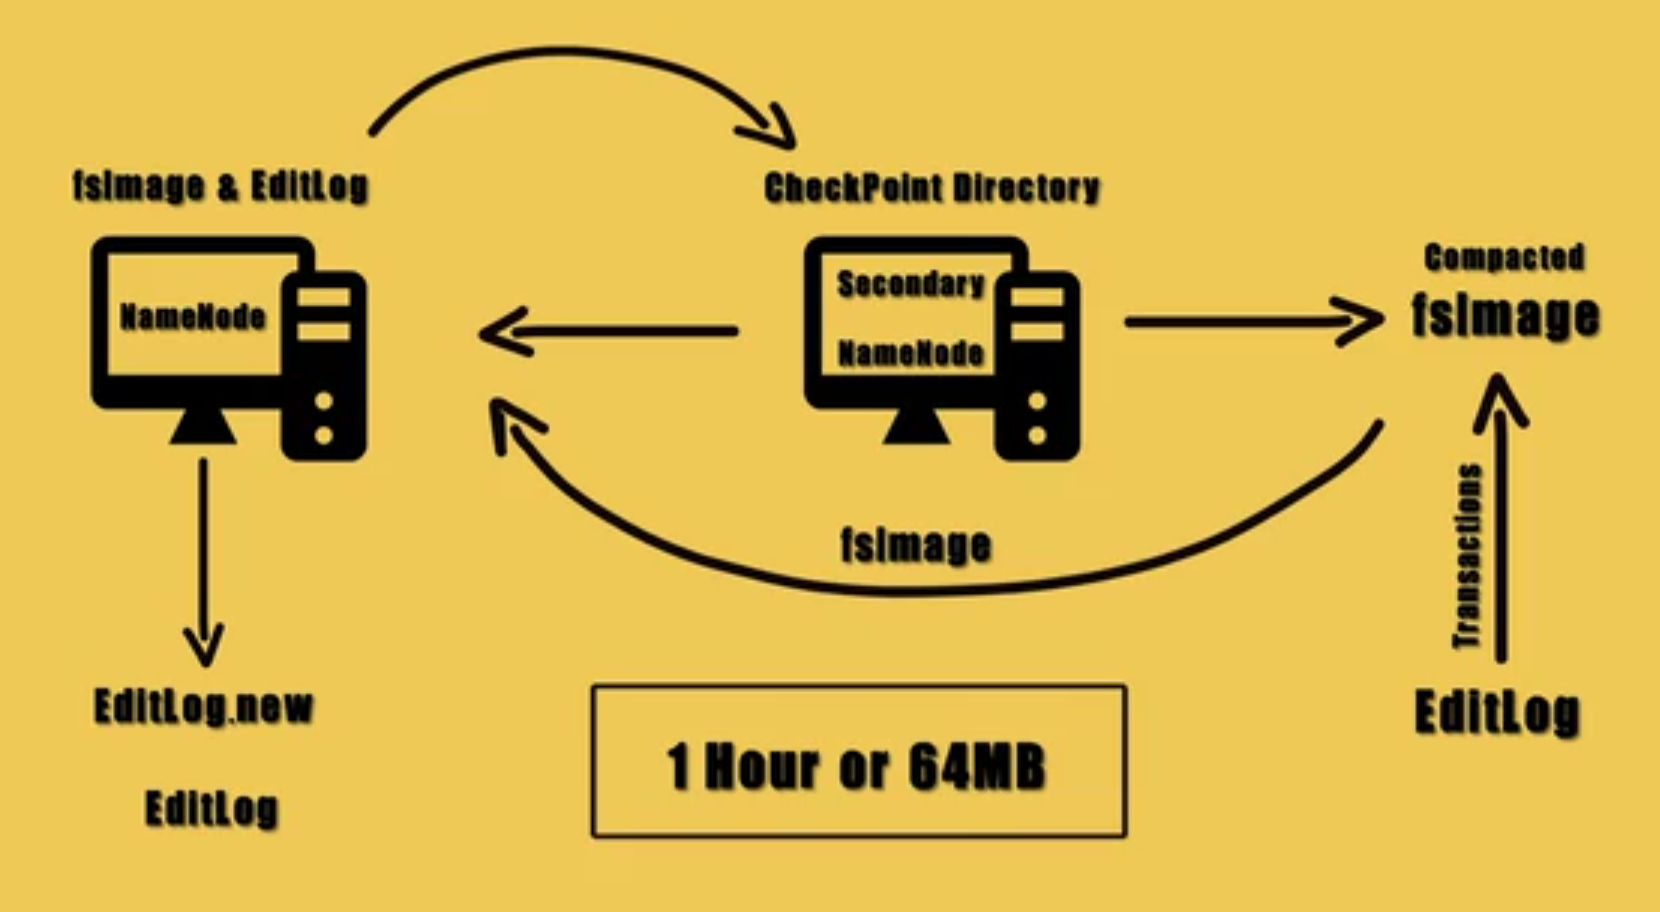
\includegraphics[scale=0.30]{Gambar/IX-Secondary-NameNode}
			%\caption[Alur kerja Secondary NameNode dan NameNode]{Alur kerja Secondary NameNode dan NameNode} 
			%\label{fig:IX-Secondary-NameNode}
			%\end{figure}

			Secondary NameNode merupakan MasterNode cadangan yang selalu aktif mencatat seluruh kegiatan dari NameNode untuk menjadi backup apabila server masternode yang utama mengalami kendala. Setiap transaksi yang dilakukan dicatat di dalam file editLog \footnote{File editLog adalah file yang menyimpan seluruh modifikasi yang dilakukan terhadap metadata}. Secondary NameNode memeriksa NameNode untuk menyimpan transaksi terbaru pada file editlog yang baru. Secondary NameNode membuat salinan dari fsImage \footnote{fsImage adalah file yang berisi snapshot lengkap mengenai metadata. Menyimpan semua blok yang dimiliki oleh suatu file dan file system property} dan editLog pada direktori \textit{checkpoint}. Setelah itu, ia menyimpan transaksi terbaru yang terjadi pada file editLog dan menyimpan seluruh informasi yang terbaru ke dalam \textit{compacted fsImage} baru. Secondary NameNode mengirim fsImage yang baru tersebut ke NameNode dan NameNode memilih fsImage yang baru tersebut. Proses ini berjalan setiap 1 jam sekali atau ketika besaran dari file editLog sudah mencapai 64MB. 
			Seperti yang tertera pada gambar 2.2. Ketika NameNode baru dijalankan, ia membuat file fsImage dan file editLog dari disk. Lalu menuliskan semua transaksi ke dalam metadata dari editLog yang telah di salin ke dalam RAM. Setelah selesai, versi baru dari fsImage dikembalikan dari memori RAM kepada memori disk.
		\end{enumerate}		
		
			%\begin{figure}
			%\centering
			%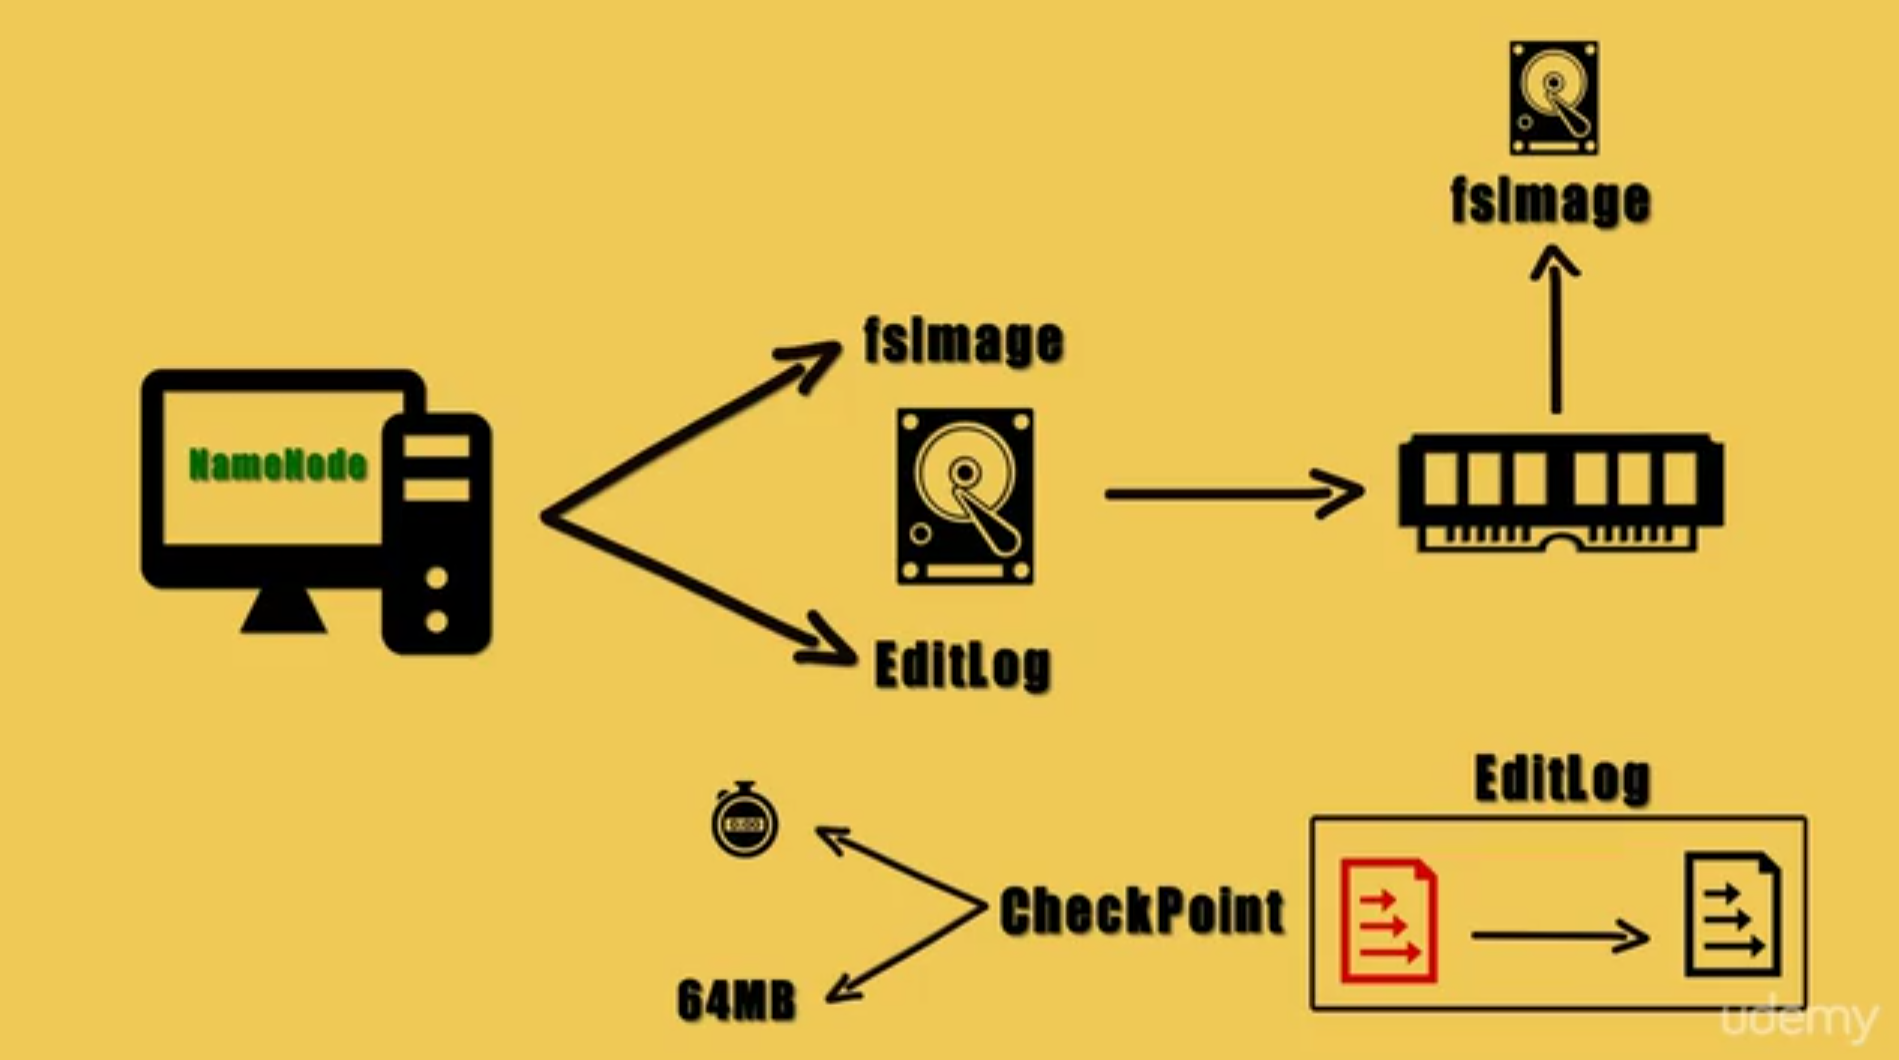
\includegraphics[scale=0.2]{Gambar/X-FileSystem-Metadata}
			%\caption[FileSystem Metadata pada NameNode dan Secondary NameNode]{FileSystem Metadata on NameNode and Secondary NameNode}
			%\label{fig:X-FileSystem-Metadata}
			%\end{figure}
			
			\begin{figure}[ht]
			\centering
			\includegraphics[scale=0.5]{GambarIO/X-FileSystem-Metadata}
			\caption[FileSystem Metadata pada NameNode dan Secondary NameNode]{FileSystem Metadata pada NameNode dan Secondary NameNode}
			\label{fig:FileSystem Metadata pada NameNode dan Secondary NameNode}
			\end{figure}
			
			HDFS memiliki 2 operasi yang penting, yaitu operasi baca dan operasi tulis dari dan ke HDFS. Berikut merupakan penjelasan lebih lanjut mengenai operasi baca dan operasi tulis dari dan ke HDFS.
		
		\paragraph{Membaca data dari HDFS}
			Untuk dapat membaca data dari HDFS, Hadoop Client membutuhkan "Hadoop Client Library" dan konfigurasi dari cluster. Mekanisme operasi baca data dari HDFS adalah sebagai berikut : (Ilustrasi pada gambar 2.4) : 
			
			\begin{figure}[ht]
			\centering
			\includegraphics[scale=0.54]{GambarIO/XI-Client-read-data-from-HDFS}
			\caption[Client membaca data dari HDFS]{Client membaca data dari HDFS}
			\label{fig:XI-Client-read-data-from-HDFS}
			\end{figure}
			
			%\begin{figure}
			%\centering
			%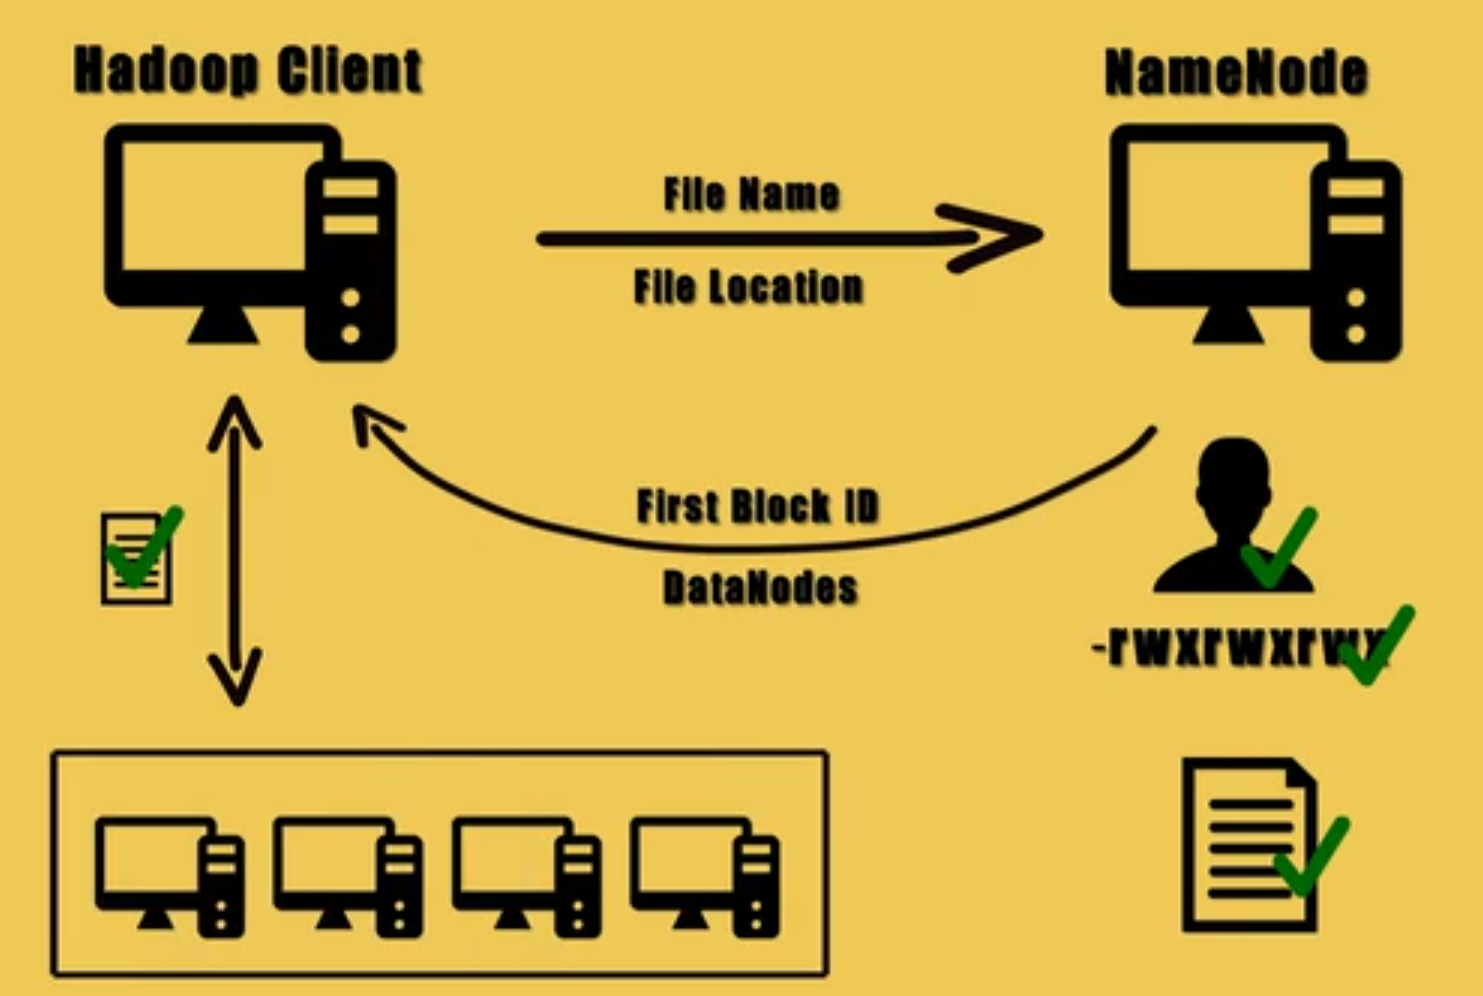
\includegraphics[scale=0.30]{Gambar/XI-Client-read-data-from-HDFS}
			%\caption[Client membaca data dari HDFS]{Client membaca data dari HDFS}
			%\label{fig:XI-Client-read-data-from-HDFS}
			%\end{figure}
			
			\begin{enumerate}
				\item Client menghubungi NameNode dan memberikan nama file pada file yang ingin dibaca.
				\item NameNode memvalidasi client untuk memeriksa permission yang dimiliki oleh user tersebut terhadap file yang diminta. 
				\item NameNode memberikan respon kembali kepada client dengan memberikan \textit{first block ID} \footnote{First block ID merepresentasikan tempat penyimpanan 64MB pertama dari data yang diminta tersebut. Memberikan informasi seperti pada rak dan DataNode yang menyimpan blok pertama pada file yang diminta.} dengan seluruh DataNode yang memiliki salinan/replikasi dari file yang dimintanya tersebut.
				\item Setiap DataNode yang memiliki salinan diurutkan berdasarkan yang terdekat sebelum dikirimkan kepada client.
				\item Setelah informasi - informasi di atas diterima oleh client, client dapat menghubungi secara langsung DataNode yang berhubungan dan membaca file nya.
				\item Jika DataNode yang digunakan pada saat melakukan operasi baca ke HDFS mengalami kerusakan, maka client langsung mengarahkan pembacaan ke DataNode yang lainnya yang memiliki replikasi dari data tersebut. Ilustrasi pada gambar 2.5.
				\item Jika replikasi yang dibutuhkan pada DataNode lainnya tidak ada, maka operasi baca mengalami kagagalan \textit{fail}. Ilustrasi pada gambar 2.6.
				
			\begin{figure}[h]
				\centering
				\includegraphics[scale=0.50]{GambarIO/Failure-Takeover-1}
				\caption[Failure takeover 1]{Failure takeover (success scheme)}
				\label{fig:Failure takeover (success scheme)}
			\end{figure}
			
			\begin{figure}[h]
				\centering
				\includegraphics[scale=0.50]{GambarIO/Failure-Takeover-2}
				\caption[Failure takeover 1]{Failure takeover (failure scheme)}
				\label{fig:Failure takeover (failure scheme)}
			\end{figure}
				
			\end{enumerate}		
		\paragraph{Menulis data ke HDFS}
		Gambar 2.6
		Mekanisme operasi tulis ke dalam HDFS :
		
		\begin{figure}[ht]
			\centering
			\includegraphics[scale=0.5]{GambarIO/XII-Client-Writing-data-on-to-HDFS}
			\caption[Client menulis data ke HDFS]{Client menulis data ke HDFS}
			\label{fig:XII-Client-Writing-data-on-to-HDFS}
		\end{figure}
			
		%\begin{figure}
			%\centering
			%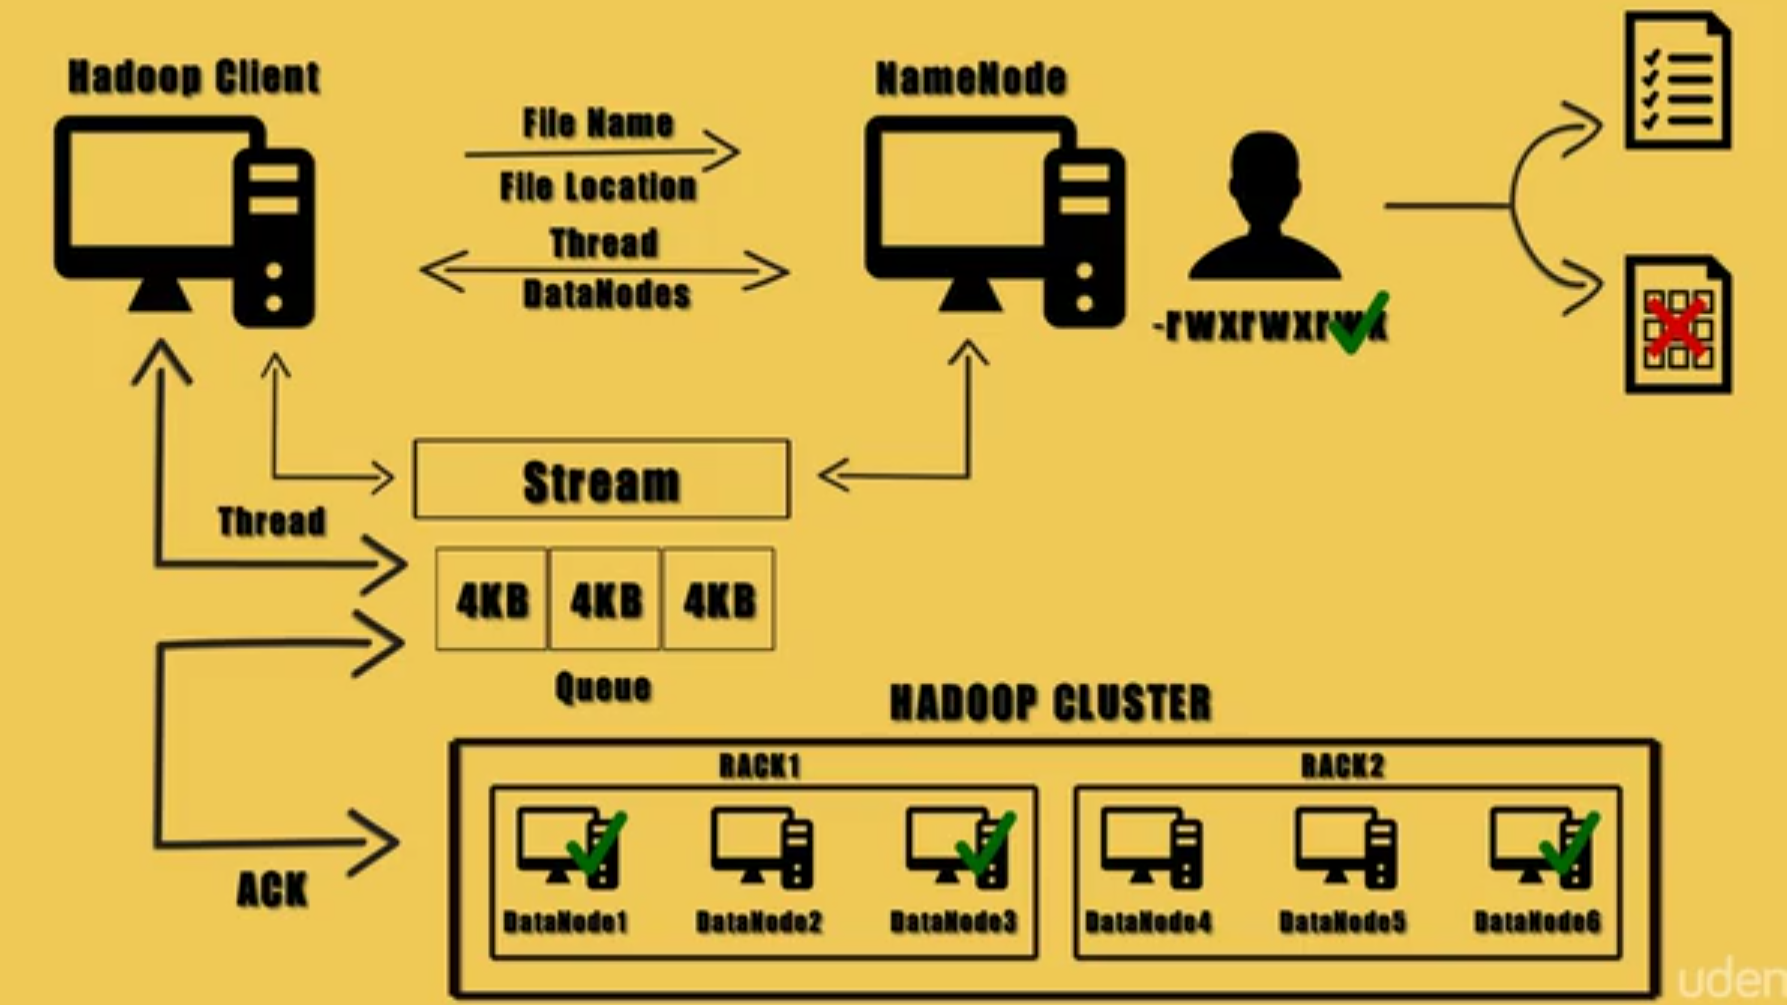
\includegraphics[scale=0.30]{Gambar/XII-Client-Writing-data-on-to-HDFS}
			%\caption[Client menulis data ke HDFS]{Client menulis data ke HDFS}
			%\label{fig:XII-Client-Writing-data-on-to-HDFS}
			%\end{figure}
			
		\begin{enumerate}
			\item Client menghubungi NameNode dan memberikan nama file dan lokasi yang diinginkan dari file yang ditulis.
			\item NameNode memvalidasi client untuk memeriksa permission yang dimiliki oleh user tersebut terhadap lokasi untuk penulisan file tersebut.
			\item NameNode membukakan sebuah stream untuk client melakukan operasi tulis. Data yang ditulis pada stream dipecah menjadi bagian - bagian kecil yang berukuran 4KB dan disimpan ke dalam queue.
			\item Client membuka thread yang berbeda yang bertanggung jawab untuk menuliskan data dari queue ke dalam HDFS.
			\item Thread menghubungi NameNode untuk meminta list dari DataNode yang dibutuhkan untuk menyalin replikasi dari data baru ini.
			\item Client menghubungi secara langsung DataNode pertama dan melakukan penulisan hingga sukses.
			\item Setelah sukses, tahap tersebut diulangi untuk setiap node yang mereplikasi data tersebut yang diberikan dari NameNode.
			\item Setelah selesai, ACK\footnote{ACK merupakan sinyal yang dikirim dalam proses komunikasi sebagai tanggapan(\textit{response}) pada protokol komunikasi.} (\textit{Acknowledgment}) diberikan kepada client untuk memberi informasi bahwa penulisan telah selesai dan berhasil.
			\item Jika ketika sedang penulisan telah mencapai maksimum dari block size, maka client kembali menghubungi NameNode untuk meminta kumpulan DataNode berikutnya yang dapat dilakukan operasi tulis.
			\item Jika telah selesai, maka client menutup stream, lalu queue dibersihkan kembali, dan metada dari NameNode diupdate.
			\item Jika pada saat penulisan terjadi kegagalan, maka data yang dikirimkan setelah ACK terakhir yang diterima oleh client dikembalikan ke queue. Lalu didelegasikan ke DataNode yang baru dengan block id yang baru.
		\end{enumerate}
		
		%HDFS memiliki satu \textit{NameNode} untuk mengatur seluruh file system metadata dan beberapa \textit{DataNodes} untuk menyimpan dataset yang sudah ter-partisi (direpresentasikan sebagai b1,b2,b3,dst.). \\
		%Ketika sekumpulan dataset masuk kedalam HDFS, HDFS mendistribusikan penyimpanan data pada tiap cluster yang berhubungan agar data tidak bercampur aduk dan dapat diambil dengan cepat. Biasanya HDFS memiliki blok data sebesar 64-128MB dan setiap partisi-nya di copy/replika-kan ke beberapa node secara acak, agar jika terjadi kegagalan dapat dengan cepat di-\textit{handle} dengan mesin lainnya.
		
%\begin{figure}
%\centering
%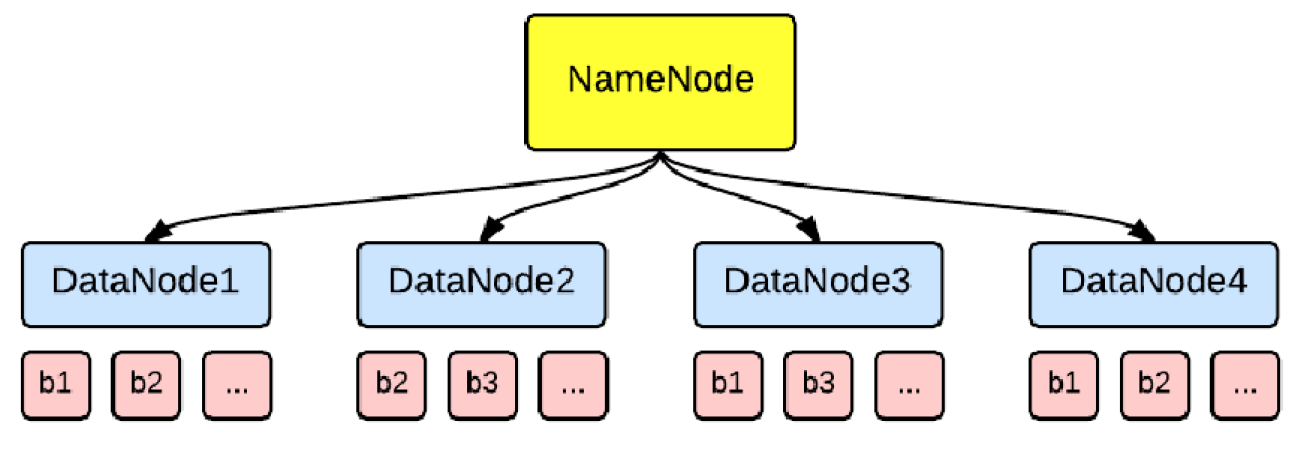
\includegraphics[scale=0.38]{Gambar/hdfs_arch}
%\caption[Arsitektur Hadoop Distributed File System (HDFS)]{Arsitektur Hadoop Distributed File System (HDFS)} 
%\label{fig:hdfs_arch}
%\end{figure}
				
\subsubsection{MapReduce}

\begin{figure}[h]
	\centering
	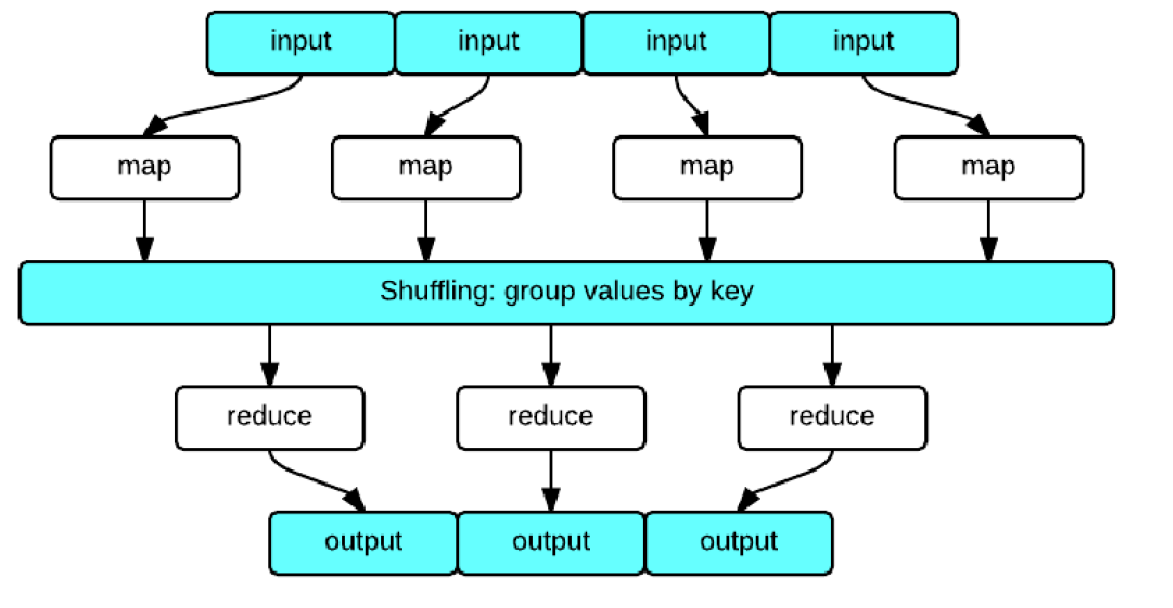
\includegraphics[scale=0.43]{GambarIO/map_reduce}
	\caption[Ilustrasi framework MapReduce]{Ilustrasi framework MapReduce}
	\label{fig:map_reduce}
\end{figure}
		
		MapReduce merupakan framework yang dirancang untuk memproses data secara paralel terdistribusi di dalam Hadoop yang memiliki performa dan efisiensi yang optimal untuk menangani data yang berukuran besar. Jenis pekerjaan pada fase map dan reduce yang dapat dikerjakan oleh framework ini merupakan jenis pekerjaan yang tidak memiliki hubungan berkesinambungan di antara  tiap proses-nya, sehingga dapat berjalan secara bersama - sama (\textit{concurrent}). Hadoop membagi/memecah seluruh dataset yang ada ke dalam beberapa partisi dan mendistribusikannya ke dalam kelompok/\textit{cluster}. MapReduce memproses data di setiap server terhadap blok - blok data yang sudah dibagikan sebelumnya, sehingga sangat menghemat waktu pekerjaan yang dihabiskan \cite{Lam:2010:HA:1965594}. \\
		Terdapat 3 fase utama dan 1 fase yang opsional(bisa dijalankan atau tidak, bergantung pada kebutuhan) pada MapReduce, yaitu fase \textit{map}, fase \textit{shuffle}, fase \textit{reduce}, dan fase \textit{combine}. 
		\begin{enumerate}
			\item Pada fase \textit{map}, melakukan konversi tiap partisi dari input ke dalam pasangan \textit{key/value} (seperti pada struktur data HashMap) lalu menggabungkan setiap \textit{value} yang memiliki \textit{key} yang sama.
			\item Pada fase shuffle, hasil keluaran dari fase Map di urutkan berdasarkan key dan pasangan \textit{key/value} tersebut dikirimkan ke reducer node yang menerima pasangan \textit{key/value} yang sesuai.
			\item Pada fase \textit{reduce}, algoritma menerima sebuah pasangan key dengan himpunan dari value yang memiliki hubungan dengan key tersebut, lalu melakukan suatu proses yang nantinya menjadi keluaran dari program MapReduce.
			\item Fase \textit{combine} ini merupakan fase yang sifatnya opsional, bisa dijalankan atau tidak. Fase ini akan melakukan yang sama seperti pada fase \textit{reduce}, hanya saja dijalankan langsung setelah fase map selesai pada node yang menjalankan proses fase \textit{map} tersebut. Hal ini bertujuan agar besaran data yang dikirim dari \textit{node} pekerja pada fase \textit{map} kepada node pekerja pada fase \textit{reduce} tidak terlalu besar, karena sebelum dikirim telah dilakukan integrasi terlebih dahulu pada data yang memiliki key yang sama. Sehingga akan menghemat \textit{bandwidth} jaringan yang digunakan.
		\end{enumerate} 
		
	Beberapa komponen utama dari \textit{MapReduce} terdiri dari \textit{JobTracker} dan \textit{TaskTracker}.
	\begin{itemize}
		\item \textit{JobTracker} berperan sebagai \textit{master} dari \textit{MapReduce}. \textit{JobTracker} mengelola pekerjaan dan sumber daya dalam \textit{cluster} (\textit{TaskTracker}). \textit{JobTracker} berusaha untuk menjadwalkan proses setiap \textit{map} dan \textit{reduce} pada \textit{TaskTracker} sedekat mungkin dengan \textit{DataNode} yang memiliki blok data yang diproses.
		\item \textit{TaskTracker} adalah slave yang ada pada setiap node. \textit{TaskTracker} bertanggung jawab untuk menjalankan proses \textit{map} dan \textit{reduce} seperti yang diperintahkan oleh \textit{JobTracker}.
	\end{itemize}
		
		Komponen utama lainnya setelah release versi terbaru Hadoop 2 dari MapReduce adalah Apache YARN (\textit{Yet Another Resource Negotiator}). YARN bertanggung jawab untuk mengawasi \textit{resource} yang tersedia pada seluruh node dan memantau status dari setiap \textit{TaskTracker} yang ada pada setiap node dan status dari pekerjaannya. YARN sebagai arsitektur baru dari Apache Hadoop 2 membagi dua fungsi utama dari JobTracker/TaskTracker pada MapReduce menjadi beberapa entitas yang terpisah, diantaranya adalah: 
		\begin{itemize}
			\item \textit{Resource Manager} di \textit{node master}, yang bertugas untuk mengawasi dan mengatur seluruh \textit{resource} yang tersedia dan digunakan pada seluruh node.
			\item \textit{Application Master} di setiap aplikasi, yang berfungsi untuk memantau status dari setiap \textit{TaskTracker} yang ada pada setiap node dan status dari pekerjaannya dan juga untuk negosiasi resource dengan \textit{ResourceManager} dan kemudian bekerja sama dengan \textit{NodeManager} untuk mengeksekusi dan memonitor \textit{tasks}.
			\item \textit{NodeManager} pada setiap \textit{node slave}, yang bertanggung jawab terhadap \textit{Container}, dengan memantau penggunaan resource/sumber daya dari container(cpu, memori, disk, jaringan ) dan melaporkannya pada ResourceManager.
			\item \textit{Container} di setiap aplikasi yang jalan di \textit{NodeManager}, sebagai wadah penyimpanan data/file.
		\end{itemize}
		
\begin{figure}[H]
\centering
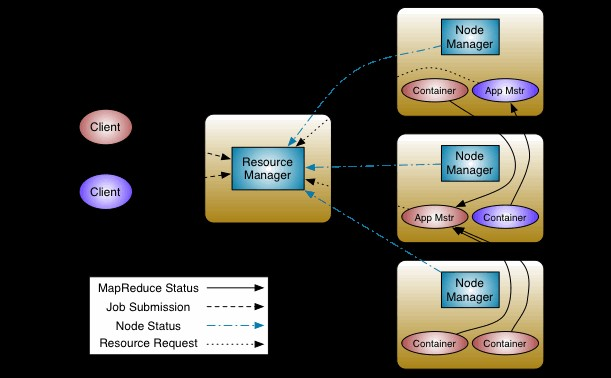
\includegraphics[scale=0.6]{YARN-Architecture}
\caption[Arsitektur YARN]{Arsitektur YARN}
\label{fig:Arsitektur YARN-1}
\end{figure}
		
Pada YARN setiap pekerjaan memiliki JobTracker-nya masing - masing dan pada suatu cluster dapat memiliki beberapa JobTracker yang sedang bekerja. Setiap JobTracker pada node yang berbeda bisa berjalan pada software yang berbeda. Hal ini yang mendukung model  dari \textit{Heterogeneous Cluster}.

%\begin{figure}[ht]
%\centering
%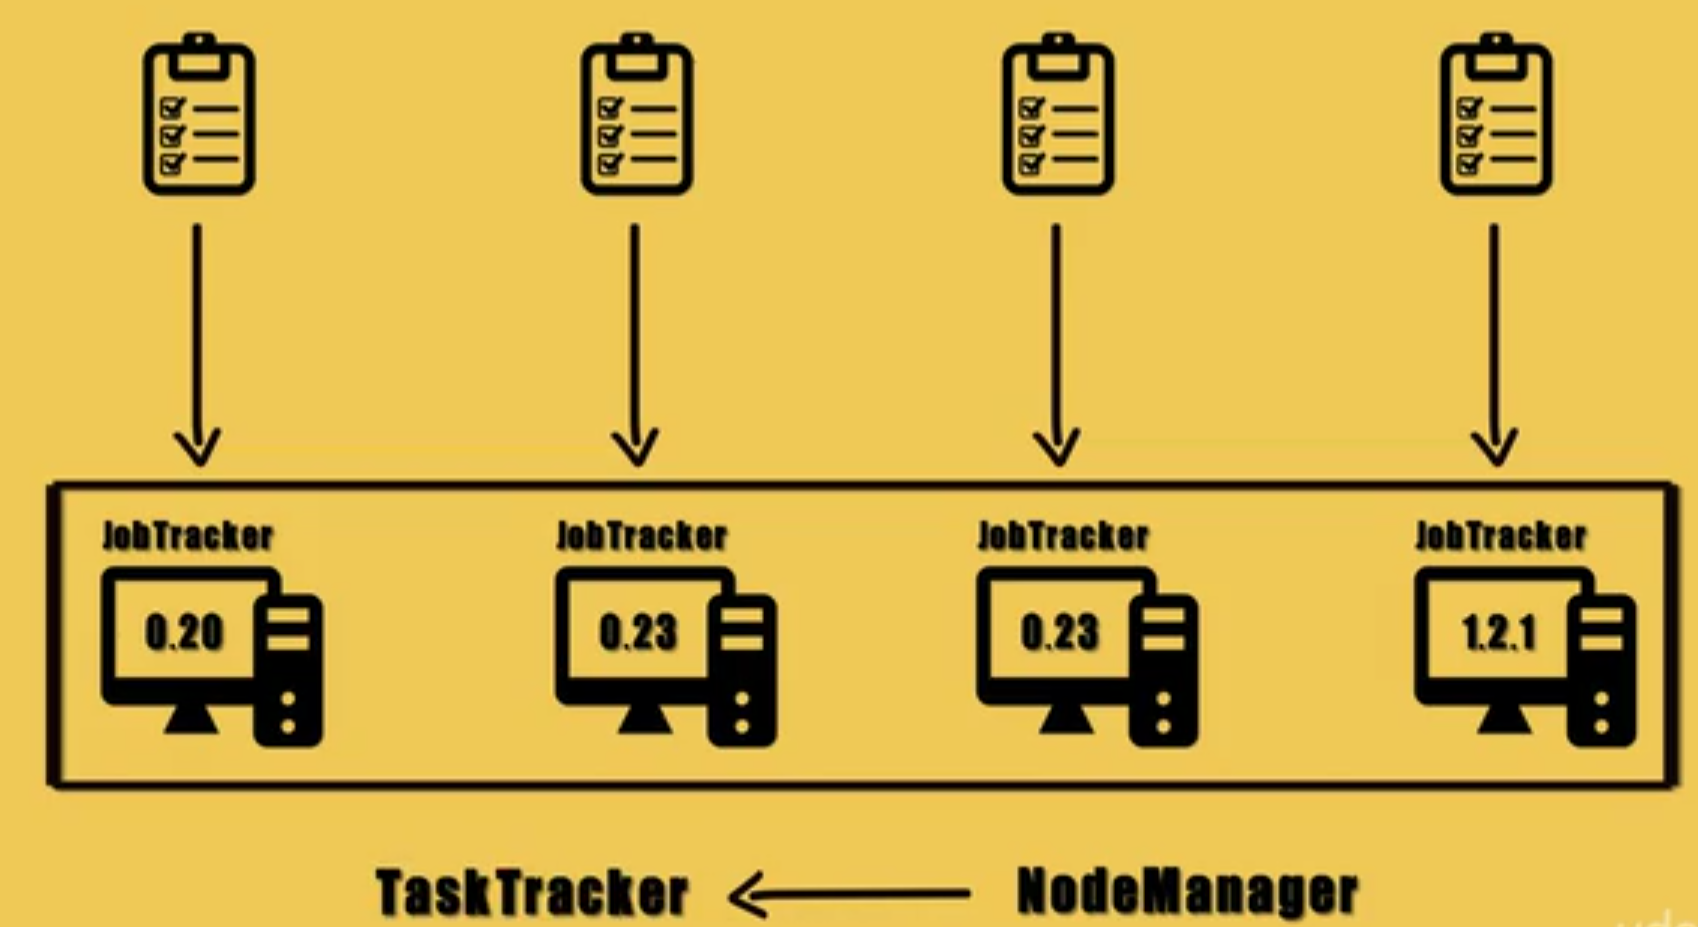
\includegraphics[scale=0.2]{Gambar/II-YARN-3-Het-Cluster}
%\caption[Arsitektur YARN-2]{Arsitektur YARN-2}
%\label{fig:Arsitektur YARN-2}
%\end{figure} 

\begin{figure}[h]
	\centering
	\includegraphics[scale=0.5]{GambarIO/Hetergenous-Cluster-YARN}
	\caption[Arsitektur YARN]{Arsitektur YARN : Heterogenous Cluster YARN}
	\label{fig:Arsitektur YARN : Heterogenous Cluster YARN}
\end{figure}

Map-Reduce ada pada setiap DataNode pada cluster Hadoop. Setiap program Map-Reduce mengerjakan atau mengolah data - data yang terdapat pada DataNode-nya. Map-Reduce ditulis dengan bahasa Java, sehingga untuk setiap abstraksi dan aturan pada pembuatan kode mengikuti bahasa Java. Selain itu, Map-Reduce milik Hadoop dibuat untuk memudahkan programmer sehingga hanya perlu berfokus pada dua buah fase yang digunakan saja, yaitu fase map dan reduce. Sedangkan untuk fase Shuffle dan Sort sudah ditangani secara otomatis oleh framework Hadoop. Berikut merupakan penjelasan lebih lanjut mengenai mapper dan reducer yang digunakan pada fase map dan fase reduce.

\paragraph{Mapper} 

Mapper berfungsi untuk memetakan data yang diberikan kepada MapReduce. Dalam Hadoop, Mapper berada pada setiap node dan bekerja menggunakan data yang berada pada masing-masing node. Hal ini dapat mengurangi lalulintas data yang terjadi pada cluster Hadoop karena tidak ada perpindahan data antar node. Mapper membaca data dalam bentuk pasangan key dengan value dan mengeluarkan nol atau lebih pasangan key dengan value dalam bentuk list yang disimpan pada penyimpanan local di DataNode (bukan dalam bentuk HDFS).

\paragraph{Reducer}

Reducer berfungsi untuk mengurangi data yang tidak diperlukan (misal : data yang berulang) atau menyatukan data yang dapat disatukan dari hasil Mapper. Jumlah Reducer pada sebuah MapReduce pada sebuah node dapat lebih dari satu. Reducer menerima sebuah list pasangan key dengan value dari Mapper yang terurut berdasarkan keynya. Hasil keluaran dari Reducer berupa nol atau lebih pasangan key dan value yang sudah final. Hasil tersebut sudah disimpan di HDFS. Sebelum diterima oleh Reducer, seluruh hasil dari Mapper melalui sebuah tahap yang dinamakan shuffle and sort. Tujuan dari tahap ini adalah memastikan bahwa semua value dengan key yang sama masuk ke reducer yang sama dan list pasangan key dan value yang diterima terurut pada berdasarkan key.

\paragraph{Cara kerja MapReduce}

%\begin{figure}[h]
%\centering
%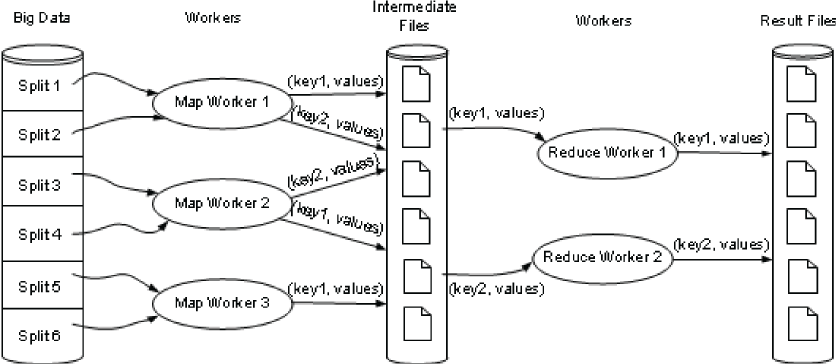
\includegraphics[scale=0.35]{Gambar/MapReduceWorks-google}
%\caption[MapReduce Works]{MapReduce Works}
%\label{fig:MapReduce Works}
%\end{figure}

\begin{enumerate}
	\item MapReduce membaca setiap line dari input yang dijadikan sebagai input dari fase Map. Setiap line yang dibaca oleh fase Map merupakan pasangan \textit{key/value} dari line yang menjadi input tersebut (sebagai value) dan offset dari text tersebut terhadap awal file (sebagai key).
	\item Fase map dijalankan sesuai apa yang kita perintahkan/implementasikan pada program Map yang dibuat. Keluaran dari fase Map merupakan pasangan \textit{key/value} yang telah diproses.
	\item Keluaran dari fungsi map sebelum dijadikan sebagai hasil input dari fungsi reduce diproses oleh fase \textit{Shuffle and Sort}. Pada fase Shuffle and Sort, hasil keluaran dari fungsi map diakumulasi dan pengurutan. Untuk setiap key yang sama dikelompokan kedalam sebuah pasangan \textit{key/value} baru yang isinya merupakan key dari input tersebut dan value nya merupakan list dari seluruh pasangan \textit{key/value} yang memiliki key sama.
	\item Setelah output fungsi map melewati proses shuffle and sort, maka output tersebut terurut berdasarkan key. Sehingga, reducer dengan tepat melihat key dan seluruh value yang bersangkutan, yang sudah ditetapkan untuk diproses pada reducer node yang menjalankan tugasnya.
	\item Pada fase reduce, dijalankan fungsi reduce yang sudah diimplementasikan sebelumnya untuk memproses pasangan dari \textit{key/list-of-value-key} menjadi hasil yang dibutuhkan.
\end{enumerate}

\begin{figure}[H]
\centering
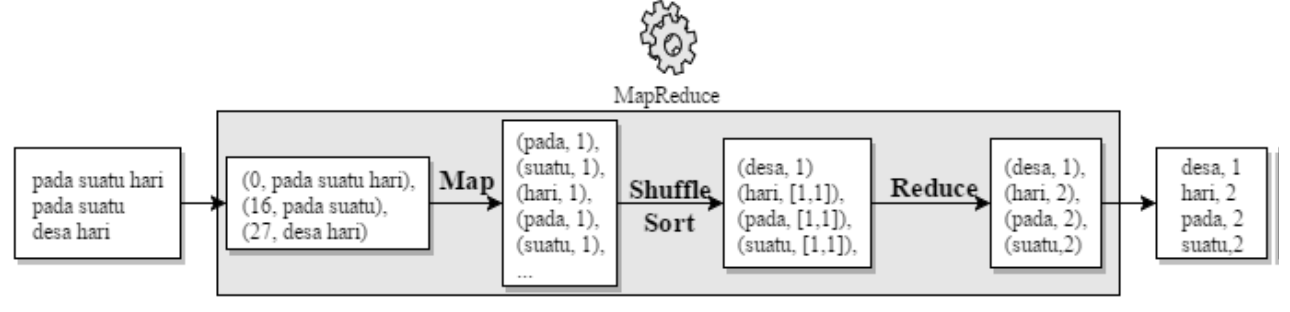
\includegraphics[scale=0.5]{contoh_mapreduce}
\caption[Proses MapReduce]{Proses MapReduce}
\label{fig:Proses MapReduce}
\end{figure}

Misalkan sebuah contoh kasus MapReduce berdasarkan Gambar~\ref{fig:Proses MapReduce}. Contoh di atas merupakan sebuah skenario program MapReduce yang melakukan perhitungan banyaknya kemunculan kata pada sebuah dokumen. Data mentah yang berasal dari HDFS mula-mula diambil per barisnya menjadi pasangan key-value yang diumpankan ke fungsi map. Pada state kedua saat pertama kali masuk ke dalam MapReduce, nilai (0, pada suatu hari), (16, pada suatu), (27, desa hari) menyatakan pasangan key-value yang diumpankan ke fungsi map. 0, 16, dan 27 menyatakan ofset data pasangan valuenya berdasarkan awal dari file HDFS. Maksudnya adalah untuk offset ke-0 value yang diumpankan adalah "pada suatu hari", mulai offset ke-16 value yang diumpankan adalah "pada suatu", dan pada offset ke 27-value yang diumpankan adalah desa. Untuk kasus ini, fungsi map diatur sedemikian sehingga menghasilkan pasangan key-value dengan key berupa sebuah kata dan value merupakan sebuah angka satu yang melambangkan kata tersebut muncul satu kali. Dapat diperhatikan juga bahwa ada pasangan key-value yang berulang seperti (pada, 1) karena pada input terdapat lebih dari satu kali kata "pada".

\begin{figure}[H]
\centering
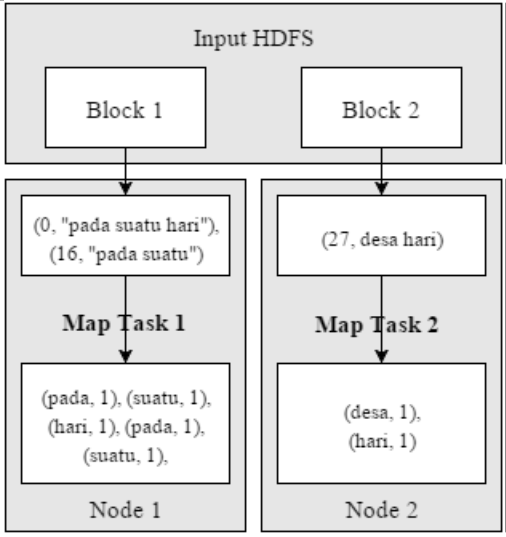
\includegraphics[scale=0.5]{proses_map}
\caption[Proses Map]{Proses Map}
\label{fig:Proses Map}
\end{figure}

Pada Gambar~\ref{fig:Proses Map}, digambarkan bila terdapat dua buah node pada sebuah cluster. File dibagi menjadi dua block dimana pada block pertama data adalah data dengan key 0 dan 16, sedangkan pada block yang ke dua adalah data dengan key 27. Kedua block tersebut masuk ke dua buah node yang berbeda, lalu dilakukan fungsi map yang terpisah dan hasilnya disimpan sementara di masing-masing node tersebut.

Setiap kunci ditetapkan pada sebuah partisi oleh sebuah komponen dalam MapReduce bernama partitioner. Di MapReduce pada Hadoop, partitioner secara default melakukan hash partition yang mengambil hash dari key yang di modulo jumlah reduce yang dikonfigurasi dalam sebuah job untuk mendapatkan nomor partisi. Pelaksanaan hash yang digunakan oleh Hadoop memastikan bahwa hash dari sebuah kunci "pada" selalu sama pada semua node yang memiliki kunci "pada". Hal tersebut menyebabkan bahwa semua "pada" ditempatkan di partisi yang sama.

Hasil keluaran dari fungsi map terlebih dahulu diolah dalam sebuah proses yang dinamakan Shuffle and Sort sebelum diumpankan selanjutnya ke fungsi reduce. Pada proses ini pasangan key-value dikelompokan dan diurutkan berdasarkan key. Proses Shuffe and Sort ini merupakan bagian pra-pengolahan data yang diumpankan pada fungsi reduce. Proses ini memiliki tujuan untuk memastikan:

\begin{itemize}
	\item Jika reducer melihat sebuah key, reducer melihat semua value untuk key tersebut. Sebagai contoh, jika sebuah key menerima kunci "pada", maka reducer menerima dua buah angka 1 sebagai value dari setiap key "pada".
	\item Sebuah kunci diproses oleh tepat satu reducer.
	\item Setiap reducer melihat key yang sudah terurut.
\end{itemize}

Pada proses Shuffle and Sort, setiap reducer pada awalnya ditetapkan sebuah partisi dimana reducer melakukan tugasnya. Pertama, reducer mengambil setiap pasangan key-value hasil dari fungsi map pada setiap node yang memiliki partisi yang ditetapkan pada reducer tersebut. Misalkan sebuah reducer yang ditetapkan mengerjakan partisi X mencari di seluruh node setiap pasangan key-value yang berada pada partisi 1. Mencari dan menduplikasi data dari setiap node menghabiskan banyak waktu dan resources yang berbanding lurus dengan jumlah data. Untuk meminimalisasi hal ini, proses pencarian dan penduplikasian data dilakukan sesegera mungkin ketika sebuah fungsi map telah selesai untuk mempersingkat runtime namun tidak dilakukan terlalu cepat karena data yang diduplikasi menyita banyak resource yang dimiliki oleh fungsi reduce bila fungsi map masih belum selesai.

\begin{figure}[H]
\centering
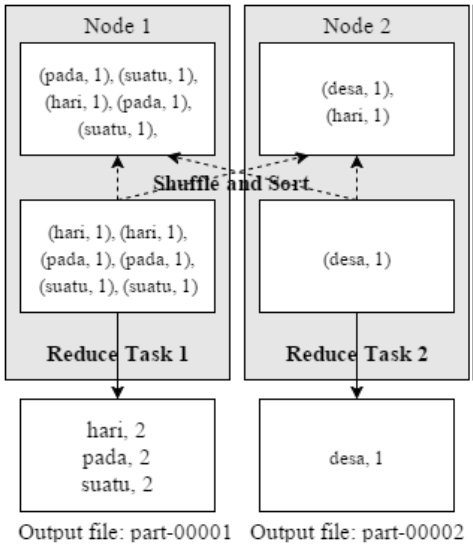
\includegraphics[scale=0.5]{proses_reduce}
\caption[Proses Reduce]{Proses Reduce}
\label{fig:Proses Reduce}
\end{figure}

Setelah data untuk fungsi reduce telah disiapkan, maka fungsi reduce sekarang dapat melakukan tugasnya. Pada kasus ini dan berdasarkan ketentuan data yang diterima sebuah reducer, misalkan sebuah reducer mendapatkan tugas untuk melakukan proses reduce pada partisi X dimana partisi tersebut berisi dua buah pasangan key-value (pada, 1) dan (di, 1). Reducer dibuat sedemikian rupa sehingga reducer menggabungkan pasangan key-value yang serupa dengan menambahkan value dari key tersebut. Untuk kasus ini maka hasil dari reducer ini berupa (pada, 2) dan (di, 1).

Setiap reducer menghasilkan output file yang berbeda antara reducer lainnya. Hal ini ditujukan agar reducer tidak harus berkoordinasi dengan reducer lainnya dalam penulisan sebuah shared file sehingga mengurangi kompleksitas dan setiap reducer bebas menyelesaikan pekerjaanya tidak bergantung dengan reducer yang lain. File yang dihasilkan biasanya dinamakan part-XXXXX dimana XXXXX merupakan penunjuk bahwa file tersebut merupakan hasil dari task reduce ke-XXXXX.
		
\section{Teorema Bayes}
	
	\cite{garg2013design} Teorema Bayes adalah salah satu teorema dalam statistika untuk menghitung peluang suatu kejadian dari beberapa kejadian lainnya. Teorema Bayes merupakan salah satu istilah dalam teori probabilitas yang berisi mengenai perhitungan probabilitas yang memiliki syarat tertentu (\textit{certain conditional probability}). Probabilitas bersyarat (\textit{conditional probabilities}) merupakan suatu probabilitas terhadap 1 kejadian tertentu yang dipengaruhi oleh probabilitas kejadian lain. Istilah yang umum digunakan pada teorema bayes adalah probabilitas \textit{prior} dan probabilitas \textit{posterior}. Probabilitas prior dari suatu kejadian(atau hipotesa) merupakan probablitas orisinil yang didapatkan sebelum dipengaruhi oleh probabilitas lain. Sedangkan probabilitas posterior merupakan probabilitas suatu kejadian yang sudah dipengaruhi oleh probabilitas dari kejadian lain.
	
	Teorema Bayes dapat ditulis sebagai:
	
\begin{equation} \label{eq:1}
P(A|B) = \dfrac{P(B|A)P(A)}{P(B)}
\end{equation}
Dimana,\\
P(A) adalah probabilitas prior dari A.\\
P(B) adalah probabilitas prior dari B.\\
P(A|B) adalah probabilitas posterior dari A jika diberikan B.\\
P(B|A) adalah probabilitas posterior dari B jika diberikan A.

\section{\textit{Naive Bayes Classifier}}
	
	 Naive Bayes merupakan salah satu metode mesin learning yang digunakan pada teknik data mining menggunakan metode perhitungan peluang. Konsep dasar yang digunakan oleh Naive bayes adalah Teorema Bayes dengan asumsi independensi\footnote{Independensi adalah keadaan bebas dari pengaruh, tidak dikendalikan oleh pihak lain.} yang kuat. \textit{Naive Bayes Classifier} pertama kali dijelaskan pada \cite{ro1973pattern} pada tahun 1973 dan setelah itu pada \cite{langley1992analysis} pada tahun 1992. Struktur dari \textit{naive bayes classifier} pertama kali digambarkan seperti pada gambar~\ref{fig:Struktur Naive Bayesian Network} yang menunjukkan asumsi independensi yang kuat antara setiap atribut(\textit{features}) pada suatu contoh data.
	 
\begin{figure}[H]
\centering
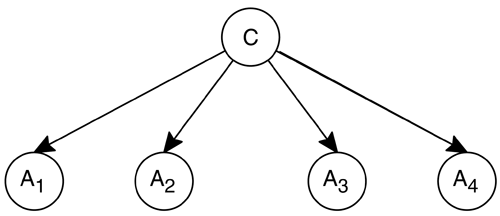
\includegraphics[scale=0.6]{naive_bayes_classifier_structure}
\caption[\textit{Bayesian Network} dengan Kedalaman 1 \textit{level}]{\textit{Bayesian Network} dengan Kedalaman 1 \textit{level}}
\label{fig:Struktur Naive Bayesian Network}
\end{figure}

	Pada Gambar~\ref{fig:Struktur Naive Bayesian Network}, $C$ melambangkan sebagai kelas dan $A_i$ melambangkan sebagai atribut - atribut yang dimiliki oleh kelas tersebut. Pada \textit{Bayesian Network} tersebut dijelaskan bahwa atribut $A_1$ sampai dengan $A_4$ akan mempengaruhi nilai dari kelas $C$, tetapi untuk setiap atribut tersebut tidak saling memiliki keterikatan dalam mempengaruhi nilai dari kelas $C$ (\textit{naive}). Oleh karena itu, pada gambar \textit{Bayesian Network}~\ref{fig:Struktur Naive Bayesian Network} hanya memiliki 1 level saja, dimana setiap atribut dalam mempengaruhi nilai kelas $C$ tidak saling memiliki keterikatan antara satu atribut dengan yang lainnya (\textit{class conditional independence}).

\subsection{Algoritma}

%	 \textit{Bayes Optimal Classifier} menghitung peluang dari satu kelas dari masing-masing kelompok atribut yang ada dan menentukan kelas mana yang paling optimal. 
	 Teori bayes memiliki asumsi bahwa probabilitas P(A|B) atau peluang kejadian A bila B terjadi tidak saling berhubungan dengan setiap kemungkinan dari nilai B yang diberikan (\textit{naive}). Hal ini disebut sebagai \textit{class conditional independence} . Sehingga memudahkan perhitungan yang dilakukan pada saat klasifikasi. Kemungkinan terjadinya kejadian A bila diberikan kejadian B dapat dihitung dengan menggunakan rumus~\ref{eq:1}, yaitu mengalikan peluang dari kejadian B jika diberikan kejadian A dikalikan dengan peluang seluruh kejadian A dan dibagi dengan peluang dari seluruh kejadian B.

	Seperti yang ditulis pada \cite{rish2001empirical}, \textit{naive bayes classifier} dapat didefinisikan sebagai berikut. Variabel - variabel dilambangkan dengan menggunakan huruf kapital seperti $X_i$, dan nilai-nya dilambangkan dengan huruf kecil seperti $x_i$, dan kumpulan dari variabel dilambangkan dengan huruf tebal seperti \textbf{$X$}.

Berdasarkan persamaan pada~\ref{eq:1}, untuk dataset $X$ dan sebuah kelas $C$, didapatkan persamaan seperti $P(C=c|X=x) = \dfrac{P(X=x|C=c)P(C=c)}{P(X=x)}$. Karena, $P(X=x)$ adalah sama untuk setiap kelas, maka bisa diabaikan. Oleh karena itu, maka fungsi diskriminan dapat ditulis menjadi $f^x = P(X=x|C=c)P(C=c)$, dimana $P(X=x|C=c)$ disebut sebagai CPD (\textit{class-conditional probability distribution}).

Untuk menghitung nilai $P(C=c|X)$ (\textit{X merupakan dataset yang digunakan sebagai predictor}) dengan mengasumsikan bahwa masing - masing atribut tidak saling bergantung dengan atribut lainnya (\textit{class conditional independence}), maka didapat : 
\begin{equation} \label{eq:2}
	P(C=c|X) = P(x_1|c) P(x_2|c) ... P(x_n|c) P(C=c)
\end{equation}

Sebuah dataset dapat ditentukan klasifikasi-nya dengan algoritma naive bayes setelah dihitung semua kemungkinan dari nilai $P(c_k|X)$ dan untuk nilai keluaran yang paling besar dipilih menjadi kelas yang paling optimal dari dataset tersebut.

\textit{MAP Maximum A Posteriori}
		\begin{equation} \label{eq:3}
			C_{MAP} = \underset{c \in C}{ argmax } P(c|X) = \underset{c \in C}{ argmax } P(X|c) P(c)
		\end{equation} \\
		
\subsubsection{Pembuatan Model}
\label{subsubsec:Pembuatan Model}

Langkah - langkah yang perlu dilakukan untuk melakukan pembuatan model adalah sebagai berikut:
\begin{enumerate}
	\item Membuat tabel frekuensi (atribut bertipe diskrit)
	\item Membuat tabel peluang (atribut bertipe diskrit)
	\item Menggunakan cara yang ada pada bagian~\ref{subsec:Prediktor Numerik} (atribut bertipe numerik)
\end{enumerate}

Dimisalkan dataset untuk contoh kasus adalah seperti berikut:

\begin{table}[H]
	\label{tab:dataset}
	\centering
	\caption{Contoh Dataset (atribut kelas = \textbf{Play})}
	\begin{tabular}{ | c | c | c | }
	\hline
	%\toprule
	Humidity & Outlook & \textbf{Play}\\ \hline \hline
	%\midrule
	60 & Rainy & No\\ \hline
	%\midrule
	78 & Rainy & No\\ \hline
	%\midrule
	80 & Sunny & Yes\\ \hline
	%\midrule
	75 & Sunny & No\\ \hline
	%\midrule
	85 & Sunny & Yes \\ \hline
	%\bottomrule
	\end{tabular}
\end{table}

Sesuai dengan langkah - langkah yang sudah dijelaskan sebelumnya, langkah pertama yang perlu dilakukan untuk membuat model naive bayes classifier adalah membuat tabel frekuensi untuk setiap atribut prediktor terhadap atribut kelas yang bertipe diskrit. Pada contoh tabel diatas, diasumsikan bahwa atribut Humidity dan Outlook merupakan atribut prediktor, lalu untuk atribut Play merupakan atribut kelas.

\begin{table}[ht]
	\centering
	\caption{Tabel frekuensi atribut Outlook}
	\label{tab:2-Table frekuensi atribut Outlook}
	\begin{tabular}{ | c | c | c | c | }
	\hline
	& \multicolumn{2}{c}{\textbf{Play}} & \\ 
	%\hline
	& Yes & No & \textit{sum} \\
	\hline
	Sunny & 2 & 1 & \textbf{3}\\
	\hline
	Rainy & 0 & 2 & \textbf{2} \\
	\hline
	\textit{sum} & \textbf{2} & \textbf{3} & \\
	\hline
	\end{tabular}
\end{table}

Pada table frekuensi untuk atribut Outlook~\ref{tab:2-Table frekuensi atribut Outlook}, dapat dilihat bahwa $P(X=Rainy|C=Yes) = 0$. Naive bayes classifier tidak dapat mengatasi frekuensi yang nilainya 0. Karena dapat menyebabkan seluruh perhitungan menjadi 0(karena berapapun bilangannya, jika dikalikan dengan 0 selalu menghasilkan nilai 0), sehingga menjadi tidak relevan. Untuk menangani hal tersebut, maka dilakukan penanganan dengan cara yang dijelaskan pada bagian~\ref{subsec:Zero-Frequency Problem}. Berdasarkan pada~\ref{subsec:Zero-Frequency Problem}, perubahan nilai atribut dapat dilihat pada Table~\ref{tab:2-Table frekuensi atribut Outlook Modif}.

\begin{table}[ht]
	\centering
	\caption{Tabel frekuensi atribut Outlook (modifikasi)}
	\label{tab:2-Table frekuensi atribut Outlook Modif}
	\begin{tabular}{|c|c|c|c|}
	\hline
	& \multicolumn{2}{c}{\textbf{Play}} & \\
	& Yes & No & \textit{sum} \\ 
	\hline
	Sunny & 3 & 2 & \textbf{5}\\
	\hline
	Rainy & 1 & 3 & \textbf{4} \\
	\hline
	\textit{sum} & \textbf{4} & \textbf{5} & \\
	\hline
	\end{tabular}
\end{table}

Langkah kedua adalah membuat tabel kemungkinan dari tabel frekuensi yang telah dibuat:		
\begin{table}[ht]
	\centering
	\caption{Tabel kemungkinan atribut Outlook}
	\begin{tabular}{|c|c|c|c|}
	\toprule
	& \multicolumn{2}{c}{\textbf{Play}} & \\
	& Yes & No & \textit{sum} \\ 
	\midrule
	Sunny & 3/4 & 2/5 & \textbf{5/9}\\
	\midrule
	Rainy & 1/4 & 3/5 & \textbf{4/9} \\
	\midrule
	\textit{sum} & \textbf{4/9} & \textbf{5/9} & \\
	\bottomrule
	\end{tabular}
\end{table}

Langkah ketiga bersifat opsional khusus untuk atribut bertipe numerik. Karena atribut Humidity bertipe numerik, atribut tersebut perlu diubah ke dalam kategori mereka masing - masing agar perhitungan dalam pembuatan model dapat tepat. Dalam melakukan pembuatan model atribut bertipe numerik, akan digunakan perhitungan standard distribusi yang dijelaskan pada bagian~\ref{subsec:Prediktor Numerik}. Berdasarkan cara pada bagian~\ref{subsec:Prediktor Numerik} perlu dibuat tabel rata - rata dan standard deviasi untuk atribut numerik terhadap setiap nilai dari atribut kelas.

		\begin{table}[H]
		\centering
		\caption{Tabel Distribusi}
		\label{tab:Table Distribusi-2}
		\begin{tabular}{|c|c|c|c|c|}
		\toprule
		\multirow{2}{*}{Play Golf ?} & Yes & 80 & 85 & \\
		 & No & 60 & 75 & 78 \\
		\bottomrule
		\end{tabular}
		\end{table}
		
		Berdasarkan Tabel Distribusi pada~\ref{tab:Table Distribusi-2}, berikut merupakan table rata - rata dan standar deviasi dari atribut Humidity yang bertipe numerik : 
		
		\begin{table}[H]
		\centering
		\caption{Tabel rata - rata dan standar deviasi atribut Humidity}
		\begin{tabular}{|c|c|c|}
		\toprule
		 & Mean & StDev \\
		Yes & 82.5 & 3.5 \\
		No & 71 & 9.6 \\
		\bottomrule
		\end{tabular}
		\end{table}



\subsubsection{Klasifikasi}
\label{subsubsec:Klasifikasi}

Setelah dilakukan pembuatan model pada bagian~\ref{subsubsec:Pembuatan Model}, klasifikasi dapat dilakukan terhadap sebuah dataset baru dengan menggunakan model yang sudah dibuat tersebut. Seperti contoh kita memiliki dua buah dataset seperti berikut:
\begin{enumerate}
	\item $X = {Humidity = 50, Outlook = Sunny}$
	\item $Y = {Humidity = 90, Outlook = Sunny}$
\end{enumerate}

Seperti yang sudah dijelaskan pada perhitungan~\ref{eq:3}, untuk dataset X dan Y perlu dicari peluang kelas yang paling tinggi. Dengan menggunakan model pada bagian~\ref{subsubsec:Pembuatan Model}, didapat bahwa:
\paragraph{Untuk dataset X dengan $P=Yes$:}
	Menghitung peluang untuk atribut $Outlook=Sunny$ dengan $P=Yes$
	\begin{equation}
			P(Outlook=Sunny|Yes) = 3/4 
			= 0.75
	\end{equation}
	
	Menghitung peluang untuk atribut $Humidity=50$ dengan $P=Yes$
		\begin{equation}
			P(Humidity=50|Yes) 
			= \dfrac{1}{\sqrt{2\pi(3.5)}}e^{-\dfrac{(\textbf{50}-82.5)^2}{2(3.5)^2}}
			= 4.031*10^{-20}
		\end{equation}
	
	\paragraph{Untuk dataset X dengan $P=No$:}
		Menghitung peluang untuk atribut $Outlook=Sunny$ dengan $P=No$
		\begin{equation}
			P(Outlook=Sunny|No) = 2/5 
			= 0.4
		\end{equation}
		Menghitung peluang untuk atribut $Humidity=50$ dengan $P=No$
		\begin{equation}
			P(Humidity=50|No) 
			= \dfrac{1}{\sqrt{2\pi(9.6)}}e^{-\dfrac{(\textbf{50}-71)^2}{2(9.6)^2}}
			= 0.011
		\end{equation}
	\paragraph{Kesimpulan untuk $dataset$ $X$}
	Dari perhitungan di atas, didapat bahwa : \\ \\
	Untuk kelas $Play=Yes$ \\
	$P(Play=Yes|X) \\
	= P(Outlook=Sunny|Play=Yes)*P(Humidity=50|Play=Yes)*P(Yes) \\
	= 0.75 * 4.031*10^{-20} * 4/9 \\
	= 1.343*10^{-20}$ \\ \\
	Untuk kelas $Play=No$ \\
	$P(Play=No|X) \\
	= P(Outlook=Sunny|Play=No)*P(Humidity=50|Play=No)*P(No) \\
	= 0.4 * 0.011 * 5/9 \\
	= 0.002$ \\ \\
	Setelah itu, lakukan normalisasi terhadap nilai - nilai berikut: \\
	$P(Play=Yes|X) = 1.343*10^{-20} / (1.343*10^{-20} + 0.002) \\
	= 6.715*10^{-18}$ \\
	$P(Play=No|X) = 0.002 / ((1.343*10^{-20}) + 0.002) \\
	= 1 (100\%)$ \\
	
	Karena, $P(Play=Yes|X) = 6.715*10^{-18} < P(Play=No|X) = 1 (100\%) $, maka hasil klasifikasi untuk \textit{dataset X} ialah kelas $Play=No$.
	
	\paragraph{Untuk dataset Y dengan $P=Yes$}
	Menghitung peluang untuk atribut $Outlook=Sunny$ dengan $P=Yes$
	\begin{equation}
			P(Outlook=Sunny|Yes) = 3/4 
			= 0.75
	\end{equation}
	
	Menghitung peluang untuk atribut $Humidity=90$ dengan $P=Yes$
		\begin{equation}
			P(Humidity=90|Yes) 
			= \dfrac{1}{\sqrt{2\pi(3.5)}}e^{-\dfrac{(\textbf{90}-82.5)^2}{2(3.5)^2}}
			= 0.021
		\end{equation}
	
	\paragraph{Untuk dataset Y dengan $P=No$:}
	Menghitung peluang untuk atribut $Outlook=Sunny$ dengan $P=No$
	\begin{equation}
				P(Outlook=Sunny|No)
				= 2/5 
				= 0.4
		\end{equation}
	
	Menghitung peluang untuk atribut $Humidity=90$ dengan $P=No$
		\begin{equation}
			P(Humidity=90|No)
			= \dfrac{1}{\sqrt{2\pi(9.6)}}e^{-\dfrac{(\textbf{90}-71)^2}{2(9.6)^2}} 
			= 0.018
		\end{equation}
		
	\paragraph{Kesimpulan untuk $dataset$ $Y$}
	Dari perhitungan di atas, didapat bahwa : \\ \\
	Untuk kelas $Play=Yes$ \\
	$P(Play=Yes|Y) \\
	= P(Outlook=Sunny|Play=Yes)*P(Humidity=90|Play=Yes)*P(Yes) \\
	= 0.75 * 0.021 * 4/9 \\
	= 0.007$ \\ \\
	Untuk kelas $Play=No$ \\
	$P(Play=No|Y) \\
	= P(Outlook=Sunny|Play=No)*P(Humidity=90|Play=No)*P(No) \\
	= 0.4 * 0.018 * 5/9 \\
	= 0.004$ \\ \\
	Setelah itu, lakukan normalisasi terhadap nilai - nilai berikut: \\
	$P(Play=Yes|Y) = 0.007 / (0.007+0.004) \\
	= 0.64 (64\%)$ \\
	$P(Play=No|Y) = 0.004 / (0.007+0.004) \\
	= 0.46 (46\%)$ \\
	
	Karena, $P(Play=Yes|Y) = 0.64 (64\%) > P(Play=No|Y) = 0.46 (46\%)$, maka hasil klasifikasi untuk \textit{dataset Y} ialah kelas $Play=Yes$.
	

%\begin{itemize}
%	\item $P(c|d)$ merupakan peluang dari kemunculan suatu kelas/kelompok tertentu jika diberikan suatu dataset $d$
%	\item $P(d|c)$ merupakan peluang suatu dataset tertentu jika diberikan suatu kelas $c$
%	\item $P(c)$ merupakan probabilitas dari kelas
%	\item $P(d)$ merupakan probabilitas dari dokumen/dataset
%\end{itemize}

\subsection{\textit{Zero-Frequency Problem}}
\label{subsec:Zero-Frequency Problem}
\cite{PeughMissing:2004} 
Ketika ada suatu nilai dari atribut prediktor yang tidak memiliki frekuensi kemunculan sama sekali terhadap setiap kelas (frekuensi=0), maka nilai 1 ditambahkan kepada setiap kombinasi dari frekuensi dari atribut terhadap tiap kelas. Pendekatan yang digunakan untuk dalam mengatasi hal ini adalah dengan menggunakan metode \textit{Laplacian Correction}. Pada metode tersebut, dikatakan bahwa kita perlu menambah nilai 1 kepada seluruh nilai pada table frekuensi untuk mengatasi masalah \textit{zero-frequency problems}. Asumsikan training database (D) itu sangat besar, dimana menambahkan frekuensi sebanyak 1 ke setiap jumlah perhitungan yang kita perlukan tidak memberikan pengaruh yang besar terhadap nilai kemungkinan akhir (Laplacian correction / Laplace estimator).

\subsection{Prediktor Numerik}
\label{subsec:Prediktor Numerik}
\cite{garg2013design} 
Ketika suatu atribut prediktor memiliki data bersifat kontinu atau numerik, terdapat 2 cara untuk mengatasi hal tersebut, diantaranya adalah:
\begin{enumerate}
	\item Melakukan transformasi atribut numerik dengan cara memecah - mecah nilai distribusi dari seluruh nilai dalam atribut tersebut ke dalam kategori - kategori terpisah. Cara tersebut disebut sebagai \textit{binning}. Cara ini perlu dilakukan sebelum membuat tabel frekuensi.
	
	\item Menggunakan disribusi dari nilai - nilai dalam atribut numerik tersebut untuk menebak frekuensi-nya. Salah satu cara yang umum digunakan adalah dengan menggunakan fungsi \textit{normal distribution} untuk nilai numerik, yang didefinisikan dengan 2 parameter: \textit{mean} dan \textit{standard deviation}.
	\begin{equation}
	P(X=x|C=c) = \dfrac{1}{\sqrt{2\pi\sigma}}\epsilon^{-\dfrac{x-\mu}{2\sigma^2}}
	\end{equation}
	Dimana,\\
	\textit{Mean} $= \mu = \dfrac{1}{n}\sum^n_{j=1}x_j$\\
	\textit{Standard Deviation} $= \sigma = [\dfrac{1}{n-1}\sum^n_{j=1}(x_j-\mu)^2]^{0.5}$\\
	\textit{n} $=$ jumlah kemunculan atribut terhadap kelas
	
	
\end{enumerate}

\subsection{Pengukuran \textit{Naive Bayes Classifier}}
\label{subsec:Pengukuran Naive Bayes Classifier}

Pengukuran dari sebuah model NBC (\textit{Naive Bayes Classifier}) dapat dilakukan dengan melihat kepada contoh tabel \textit{confusion matrix}~\ref{tab:conf_matrix}. Dapat dilihat pada tabel~\ref{tab:conf_matrix}, bahwa kolom pada \textit{confusion matrix} menyatakan nilai dari kelas hasil klasifikasi model NBC dan baris pada \textit{confusion matrix} menyatakan nilai sebenarnya dari data yang diklasifikasi. Terdapat beberapa istilah yang umum digunakan pada perhitungan model klasifikasi, diantaranya adalah sebagai berikut:
\begin{enumerate}
	\item \texttt{TP =} data yang secara benar diklasifikasikan ke dalam kategori positif.
	\item \texttt{FP =} data yang secara tidak benar diklasifikasikan ke dalam kategori positif (data sebenarnya bernilai negatif).
	\item \texttt{TN =} data yang secara benar diklasifikasikan ke dalam kategori negatif.
	\item \texttt{FN =} data yang secara tidak benar diklasifikasikan ke dalam kategori negatif (data sebenarnya bernilai positif).
\end{enumerate}

\begin{table}[h]
\centering
\caption{Contoh \textit{Confusion Matrix}}
\label{tab:conf_matrix}
\begin{tabular}{ | c | c | c | c | }
\hline
 & $Predicted=c_1$ & $Predicted=c_2$ & $Predicted=c_3$ \\ \hline \hline
$Actual=c_1$ & $r$ & $s$ & $t$ \\ \hline
$Actual=c_2$ & $u$ & $v$ & $w$ \\ \hline
$Actual=c_3$ & $x$ & $y$ & $z$ \\ \hline
\end{tabular}
\end{table}


\textit{Confusion matrix} digunakan untuk menguji model NBC yang memiliki nilai atribut lebih dari 2 (\textit{multi-class classification}). Pada \textit{confusion matrix}, terdapat beberapa perhitungan evaluasi model NBC yang dapat diperoleh dari \textit{confusion matrix}, berikut merupakan penjelasan dari tiap perhitungan evaluasi yang digunakan.
\begin{enumerate}
	\item \textit{Accuracy}\\
	\textit{Accuracy} merupakan perhitungan kesalahan sistematik untuk melakuakn evaluasi terhadap model klasifikasi. \textit{Accuracy} dapat dihasilkan dengan menghitung jumlah seluruh data yang nilai klasifikasi-nya sama dengan nilai sebenarnya pada data tersebut dibagi dengan keseluruhan dataset. Pada \textit{confusion matrix}, perhitungan \textit{accuracy} dapat dilakukan dengan menjumlahkan seluruh garis diagonal pada matrix dan membaginya dengan seluruh dataset seperti pada tabel~\ref{tab:confusion_accuracy}.
	
\begin{table}[H]
\centering
\caption{\textit{Confusion Matrix - Accuracy}}
\label{tab:confusion_accuracy}
\begin{tabular}{ | c | c | c | c | }
\hline
 & $Predicted=c_1$ & $Predicted=c_2$ & $Predicted=c_3$ \\ \hline \hline
$Actual=c_1$ & $TP$ & $s$ & $t$ \\ \hline
$Actual=c_2$ & $u$ & $TP$ & $w$ \\ \hline
$Actual=c_3$ & $x$ & $y$ & $TP$ \\ \hline
\end{tabular}
\end{table}

	 \textit{Accuracy} tidak selalu dapat diandalkan jika menghadapi sejumlah dataset yang tidak umum. Seperti contoh, pada sebuah dataset yang memiliki 2 buah kategori kelas, 100\% dari dataset tersebut berasal dari kategori A dan tidak ada yang berasal dari kategori B. Hal ini menjadikan model klasifikasi yang dibuat menjadi tidak berguna. Hal ini disebut sebagai \textit{accuracy paradox}. Ketika TP < FP, maka nilai \textit{accuracy} selalu meningkat ketika kita mengganti aturan dari klasifikasi untuk selalu mengeluarkan nilai B. Begitu juga sebaliknya, ketika TN < FN, maka hal yang sama terjadi. Untuk menangani hal tersebut, digunakan perhitungan \textit{precision}, \textit{recall}, dan \textit{f-measure} yang dijelaskan pada poin berikutnya.
	 
	 \item \textit{Precision}\\
	 \textit{Precision}(biasa disebut juga sebagai \textit{positive predictive value}) merupakan pecahan dari suatu data contoh yang relevan dan diambil terhadap seluruh data yang diambil. Pada \textit{confusion matrix} \textit{precision} dapat diperoleh dengan perhitungan berikut:

	 \begin{equation}
	 	Recall = \dfrac{TP}{(TP + FP)}
	 \end{equation}
	 
	 Dimana TP dan FP merupakan jumlah dari prediksi yang menghasilkan nilai \textit{true positive} dan \textit{false positive} pada kelas tertentu. Contoh ilustrasi pada gambar~\ref{fig:precision_recall}. 
	 
	\begin{figure}[H]
	\centering
	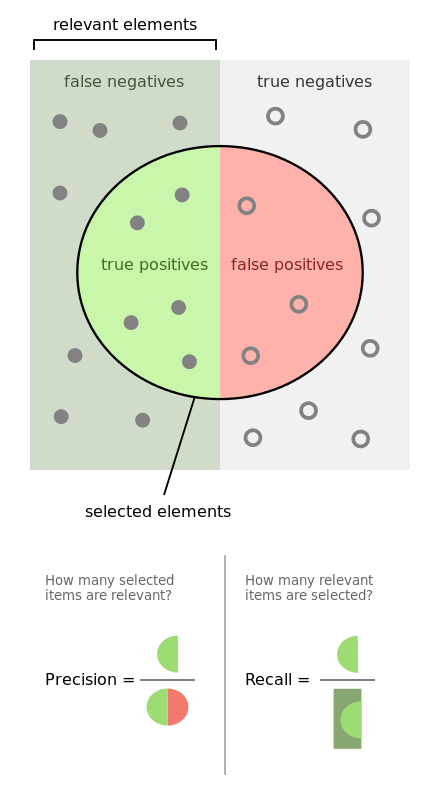
\includegraphics[scale=0.5]{precision_recall}
	\caption[\textit{Precision dan Recall}, diambil dari \url{https://en.wikipedia.org/wiki/Precision_and_recall}]{\textit{Precision dan Recall}, diambil dari \url{https://en.wikipedia.org/wiki/Precision_and_recall}}
	\label{fig:precision_recall}
\end{figure}

	 \item \textit{Recall}\\
	 \textit{Recall}(biasa disebut juga sebagai \textit{sensitivity}) merupakan pecahan dari suatu data contoh yang relevan dan diambil terhadap seluruh data yang relevan. Contoh ilustrasi pada gambar~\ref{fig:precision_recall}. Pada \textit{confusion matrix} \textit{recall} dapat diperoleh dengan perhitungan berikut:

	 \begin{equation}
	 	Recall = \dfrac{TP}{(TP + FN)}
	 \end{equation}
	Dimana TP dan FN merupakan jumlah dari prediksi yang menghasilkan nilai \textit{true positive} dan \textit{false negative} pada kelas tertentu. Contoh ilustrasi pada gambar~\ref{fig:precision_recall}. 	 
	 
	 \item \textit{F-Measure}\\
	  \textit{F-Measure} merupakan suatu pengukuran yang mengkombinasikan pengukuran \textit{precision} dan pengukuran \textit{recall}. Berdasarkan dari rumus turunan oleh \textit{van Rijsbergen's}, diperoleh perhitungan yang efektif untuk menghitung \textit{F-Measure} adalah sebagai berikut:
	 
	 \begin{equation}
	 	\dfrac{1}{\alpha \dfrac{1}{P} + (1 - \alpha)\dfrac{1}{R}}
	 \end{equation}
	 Dimana, $\alpha$ merupakan koefisien bobot dari \textit{recall} dan \textit{precision}, biasanya digunakan $balanced F1$ untuk mengisi nilai $\alpha$ :
	 \begin{equation}
	 	\dfrac{2PR}{P + R}
	 \end{equation}

\end{enumerate}


\paragraph{Pengukuran \textit{Naive Bayes Classifier} Menggunakan Model Pada~\ref{subsubsec:Pembuatan Model}}

Untuk melakukan sebuah pengukuran terhadap model NBC (\textit{Naive Bayes Classifier}), diperlukan sebuah data pelatihan yang sudah memiliki nilai asli dari atribut yang bertipe kelas. Dimisalkan kita memiliki data pelatihan seperti ini:
\begin{enumerate}
	\item $X = {Humidity = 50, Outlook = Sunny, Play = No}$
	\item $Y = {Humidity = 90, Outlook = Sunny, Play = Yes}$
\end{enumerate}

Setelah itu, untuk setiap data pelatihan tersebut, akan dilakukan perhitungan klasifikasi menggunakan cara yang sudah dijelaskan pada bagian~\ref{subsubsec:Klasifikasi}. Setelah dilakukan klasifikasi terhadap kedua data pelatihan tersebut, didapat bahwa: (1) untuk data pelatihan X memiliki hasil prediksi atribut kelas $Play = No$; (2) untuk data pelatihan Y memiliki hasil prediksi atribut kelas $Play = Yes$. Sampai dengan tahap ini, sudah didapat nilai hasil prediksi terhadap kedua data pelatihan tersebut dan nilai asli dari atribut kelas milik data pelatihan tersebut. 

Hasil prediksi klasifikasi nilai atribut kelas pada data pelatihan tersebut perlu dimasukkan kedalam \textit{confusion matrix}, dengan melakukan pencocokan terhadap tiap baris dan kolom yang ada pada \textit{confusion matrix}. Berikut merupakan \textit{confusion matrix} tersebut:

\begin{table}[h]
\centering
\caption{\textit{Confusion Matrix} Kelas Play}
\label{tab:conf_matrix_kasus}
\begin{tabular}{ | c | c | c | }
\hline
 & $(predicted)Play=Yes$ & $(predicted)Play=No$ \\ \hline \hline
$(actual)Play=Yes$ & $1$ & $0$ \\ \hline
$(actual)Play=No$ & $0$ & $1$ \\ \hline
\end{tabular}
\end{table}

Setelah selesai membuat \textit{confusion matrix} pada Tabel~\ref{tab:conf_matrix_kasus}, dapat dilakukan perhitungan untuk melakukan pengukuran menggunakan:
\begin{enumerate}
	\item \textit{Accuracy}
	\item \textit{Precision}
	\item \textit{Recall}
	\item \textit{F-Measure}
\end{enumerate}

Sampai pada tahap ini, sudah dapat dilakukan perhitungan keempat pengukuran tersebut menggunakan rumus yang sudah dijelaskan pada bagian~\ref{subsec:Pengukuran Naive Bayes Classifier}.
	
\section{Framework Yang Digunakan Dalam Membangun Perangkat Lunak}

\subsection{\textit{Spring Framework}}
\label{subsec:Spring Framework}

\textit{Spring Framework} adalah salah satu framework\footnote{framework adalah tools yang bisa digunakan untuk mengembangkan cakupan luas dari arsitektur-arsitektur yang berbeda \cite{setiawan2009pemilihan}} untuk aplikasi berbasis Java yang dapat digunakan untuk membangun sebuah aplikasi berskala besar. Model yang digunakan pada perangkat lunak yang dibangun adalah \textit{spring framework web application} yang memiliki ekstensi untuk membuat server pada aplikasi berbasis web dengan J2EE (Java 2 Enterprise Edition) \cite{SpringCommerceToha:2010}. Dengan Spring, kita bisa mengembangkan aplikasi enterprise dan berbasis web. Spring termasuk portable karena aplikasi yang dikembangkan dapat berjalan pada JVM manapun. Terdapat beberapa cara yang disediakan oleh spring untuk melakukan deploy aplikasi kita, seperti: 
\begin{enumerate}
	\item Melakukan deploy aplikasi dengan menggunakan mode standalone (menggunakan server bawaan dari \textit{spring}),
	\item Melakukan deploy aplikasi pada aplikasi server (menggunakan aplikasi web server dari luar, seperti \textit{Apache Tomcat Web Application}),
	\item Melakukan deploy aplikasi dengan menggunakan \textit{cloud PaaS}\footnote{\textit{Platform as Service} merupakan sebuah platform untuk mengembangkan, menjalankan, dan mengatur aplikasi kita tanpa melewati serangkaian konfigurasi yang rumit, layaknya \textit{dedicated server} pada umumnya} (\textit{Platform as Service}, seperti \textit{Pivotal Web Service}).
\end{enumerate}
Spring menyediakan model pemrograman terbuka yang komprehensif, kohesif, mudah dipahami serta memiliki \textit{library} yang lengkap untuk melakukan integrasi ke \textit{service - service} lain seperti \textit{Hadoop-client Library}, \textit{Mysql-connector Library}, dsb. Inti dari framework ini lebih kepada untuk membangun aplikasi web, mengatur manajemen transaksi, akses data, messaging, pengujian dsb. Kita bisa mengembangkan aplikasi web berbasis MVC dan \textit{Web-Service} framework \textit{REST-ful}\footnote{REST merupakan \textit{standard} dalam arsitektur web yang menggunakan Protocol HTTP untuk pertukaran data.  Konsep REST menekankan bahwa komunikasi yang terjadi antara \textit{client} dan \textit{server} hanya sebatas melakukan \textit{request} dan memberikan \textit{response} saja.} (\textit{Representational State Transfer}).

\textit{Design pattern} yang digunakan pada perangkat lunak yang dibuat menggunakan konsep MVC (\textit{model view controler}). Spring memiliki fitur khusus untuk membuat web berbasiskan \textit{design pattern} MVC. Berikut merupakan ilustrasi(diambil dari \url{https://docs.spring.io/spring/docs/current/spring-framework-reference/html/images/mvc.png.pagespeed.ce.tmIzOTr1gg.png}) dari \textit{request workflow} pada \textit{Spring Web} MVC.
\begin{figure}[h]
	\centering
	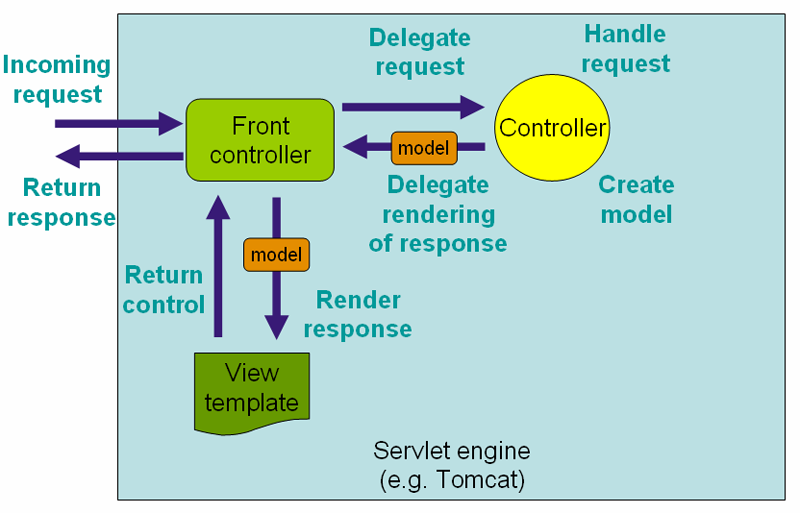
\includegraphics[scale=0.5]{GambarIO/mvc_springdocs}
	\caption[Request Processing Workflow Spring MVC]{\textit{Request Processing Workflow Spring MVC}}
	\label{fig:Request Processing Workflow Spring MVC}
\end{figure}

\begin{enumerate}
	\item \textit{\textbf{Model}} melakukan enkapsulasi dari data yang ada pada aplikasi dan secara umum berisi POJO\footnote{Istilah POJO (\textit{Plain Old Java Object}) digunakan untuk menunjukkan objek java yang hanya berisi variable serta \textit{accessor} dan \textit{mutator} -nya tanpa ada method proses lainnya}.
	
	\item \textit{\textbf{View}} bertanggung jawab untuk melakukan \textit{rendering} data dengan view HTML yang diinginkan, lalu men-\textit{generate} output berupa HTML yang dapat diinterpretasikan oleh \textit{browser}.

	\item \textit{\textbf{Controller}} bertanggung jawab untuk memproses \textit{request} dari user dan lalu perlu memberikan model sesuai dengan yang diminta yang nantinya diberikan ke \textit{view} untuk proses \textit{rendering}.
	
\end{enumerate}

%\textit{Design pattern} perangkat lunak yang dibangun mengusung konsep dari MVC milik \textit{spring} dan beberapa tambahan \textit{layer - layer} untuk mempermudah jalannya perangkat lunak nantinya. Berikut merupakan ilustrasi

\subsection{\textit{Maven}}
\cite{MengenalMaven2015EGunawan}
Apache Maven adalah software build tools / project management yang dibangun di bawah \textit{Apache Software Foundation} yang digunakan untuk melakukan proses building project. Jadi, ketika project dibuild menggunakan Maven, project tersebut bisa kita buka menggunakan IDE lain.

Selain itu, keuntungan menggunakan Maven adalah mendukung dependency management. Artinya, ketika kita membutuhkan suatu library ke dalam project, kita tidak perlu men-\textit{download}-nya secara manual yang kemudian dimasukkan ke dalam project. Tetapi, tinggal memasukkan \textit{dependency} untuk library yang dibutuhkan tersebut dan Maven menangani proses \textit{download} library dan kompilasi project menggunakan \textit{library} tersebut.  Dengan begitu, ukuran project menjadi lebih kecil karena tidak memasukkan library ke dalam project. \textit{Maven} menyimpan seluruh library yang pernah kita gunakan pada direktori \texttt{.m2} milik user.

Pada skripsi ini, Apache Maven akan digunakan untuk mempermudah penggunaan library - library yang dibutuhkan dari \textit{repository} luar seperti Hadoop Client Library dsb. pada perangkat lunak yang dibangun.

Untuk mendownload Apache Maven bisa langsung ke websitenya di \url{http://maven.apache.org/}. Versi terbaru dari Apache Maven adalah 3.5.0.

\subsection{\textit{Thymeleaf}}
\cite{CogoluegnesIntroducing:2013} 
\textit{Thymeleaf} merupakan \textit{template-engine open source} yang dapat melakukan \textit{rendering} HTML pada \textit{server-side}. Thymeleaf adalah Java XML template engine / XHTML / HTML5 yang dapat bekerja baik di web (\textit{Servlet-based}) maupun lingkungan yang bukan web. Hal ini lebih cocok untuk melayani XHTML / HTML5 pada \textit{layer} tampilan aplikasi berbasis web MVC, tetapi dapat memproses file XML bahkan di lingkungan offline. \textit{Template engine} ini menyediakan integrasi penuh dengan \textit{Spring Framework}. 

Dalam aplikasi web Thymeleaf bertujuan untuk menjadi pengganti lengkap untuk JSP, dan menerapkan konsep Natural Template: file template yang bisa langsung dibuka di browser dan yang masih menampilkan dengan benar sebagai halaman web. Sebagai \textit{framework open source}, \textit{Thymeleaf} memiliki lisensi Apache 2.0.

Pada skripsi ini, Thymeleaf akan digunakan untuk mempermudah melakukan render HTML dari data - data yang diproses oleh server dan memberikannya kepada client (untuk perangkat lunak yang dibangun berbasiskan web).


		%\paragraph{Perhitungan pada \textit{Naive Bayes Classifier}}
		%Untuk mengetahui perhitungan pada algoritma \textit{Naive Bayes}, pertama kita perlu mengetahui dan mengikuti table kontigensi 2-by-2. Terdapat 4 kondisi/\textit{state} dari setiap data yang kita evaluasi. Jika data sebenarnya merupakan instansiasi dari klasifikasi yang sedang dicoba dan klasifikasi yang kita lakukan pun menyatakan bahwa data tersebut masuk kedalam klasifikasi yang sedang dicoba, maka ia memiliki state \textit{true positive}. Jika data sebenarnya benar terklasifikasi tetapi \textit{classifier} kita mengatakan tidak, maka ia memiliki state \textit{false negative}. Jika data sebenarnya memang tidak terklasifikasi tetapi \textit{classifier} kita membuktikan bahwa data tersebut terklasifikasi, maka ia memiliki state \textit{false positive}. Dan yang terakhir adalah jika data sebenarnya tidak termasuk kedalam klasifikasi tersebut, dan \textit{classifier} kita menyatakan bahwa data tersebut memang tidak terklasifikasi, maka ia memiliki state \textit{true negative}. \\

%\begin{table}
%\centering
%\caption{The 2-by-2 contigency table}
%\begin{tabular}{c|cc}
%\toprule
% & correct & not correct\\
%\midrule
%selected & tp & fp\\
%not selected & fn & tf\\
%\bottomrule
%\end{tabular}
%\end{table}


